\documentclass[10pt,a4paper]{article}
\usepackage{mathtools}
\usepackage[T1]{fontenc}
\usepackage{lmodern}
\usepackage{textcomp}

\usepackage[english]{babel}

\usepackage{amsmath, amssymb}

\usepackage{booktabs}
\usepackage{graphicx}
\usepackage[font=small,labelfont=bf,labelsep=period,tableposition=top]{caption}
\usepackage[T1]{fontenc}
\usepackage[utf8]{inputenc}
\usepackage{amsthm}
\usepackage[]{algorithm2e}
\usepackage{xcolor}
\usepackage{listings}
\usepackage{tabularx}
\usepackage[section]{placeins}


\title{Modelli probabilistici per le decisioni: SmartHouse}
\author{Matteo Angelo Costantini, matricola: 795125 \\
	Alessandro Longhi, matricola: 794235}
\date{}
\begin{document}
	\maketitle
	\clearpage
	\tableofcontents
	\clearpage
	\section{Introduzione}
	I miglioramenti ottenuti in ambito medico hanno portato ad un sensibile aumento dell'aspettativa di vita di ogni individuo, causando un generale invecchiamento della popolazione; il quale rappresenta un importante argomento di studi nell'ambito della sanità. Infatti, aumentando il numero di individui anziani, aumenta anche la necessità di studiare e trovare una soluzione ad alcuni problemi associati alla vecchiaia.

	Focalizzarsi sui problemi dovuti all'anzianità significa, quindi, trovare dei modi efficienti per fornire supporto e cure agli individui più anziani direttamente a casa loro; tutto ciò è reso possibile grazie all'uso di sistemi di monitoraggio all'interno delle case, in quanto permettono sia l'aumento della sicurezza dell'abitante, sia il senso di protezione di quest'ultimo, favorendone l'autonomia.

	Monitorare le azioni quotidiane degli individui è uno dei task più importanti all'interno di quest'ambito, in quanto permette di descrivere il benessere degli abitanti delle case, sia fisico che mentale. Il monitoraggio delle attività avviene grazie all'uso di alcuni sensori, i quali vengono posti in diversi luoghi all'interno di ogni abitazione.

	Questo progetto si colloca nell'ambito appena descritto: avendo a disposizione dei dataset contenenti le rilevazioni delle attività e dei sensori in due abitazioni differenti, il lavoro svolto consiste nella definizione di un modello HMM in grado di inferire le attività data una sequenza di osservazioni derivanti dai sensori. Una volta creata la struttura HMM, è stata effettuata un'analisi riguardante la capacità predittiva del modello.

	La relazione verrà presentata seguendo il seguente ordine:
	\begin{itemize}
	    \item Verranno inizialmente presentati i dataset a disposizione, descrivendone anche i passaggi delle modifiche che sono state fatte al fine di semplificarne l'utilizzo
	    \item In secondo luogo, verrà discussa la creazione del modello HMM, descrivendone la creazione delle matrici necessarie per la sua definizione
	    \item Al termine di queste fasi, verrà descritta la sperimentazione svolta, alla quale seguiranno le discussioni dei risultati ottenuti
	    \item Infine, verrà presentata l'interfaccia grafica creata per effettuare i test
	\end{itemize}


	\clearpage
	\section{Analisi del dataset}
	I dataset a nostra disposizione erano quattro, due per ogni abitazione, rappresentanti rispettivamente le attività ed i sensori rilevati all'interno dell'abitazione.

	Le abitazioni considerate sono due, etichettate con "OrdonezA" ed "OrdonezB".
	\subsection{Analisi del dataset A}
	Per l'abitazione "OrdonezA" sono stati forniti due dataset: uno denominato "OrdonezA\_ADLs" contenente le attività rilevate, ed uno denominato "OrdonezA\_Sensors" contenente i sensori rilevati.
	Nel primo dataset, quello delle attività, sono descritti i seguenti campi:
	\begin{itemize}
		\item Start\_time: data ed ora di inizio della rilevazione di un'attività
		\item End\_time: data ed ora di fine della rilevazione di un'attività
		\item  Activity: attività rilevata nel periodo considerato
	\end{itemize}

	in particolare, nella colonna "Activity" sono stati rilevati 10 valori diversi, cioè: Leaving, Toileting, Showering, Sleeping, Breakfast, Lunch, Dinner, Snack, Spare\_Time/TV e Grooming.

	Il secondo dataset di "OrdonezA"è dedicato alla raccolta dei sensori rilevati. In quest'ultimo sono presenti i seguenti campi:
	\begin{itemize}
		\item Start\_time: data ed ora di inizio della rilevazione di un sensore
		\item End\_time: data ed ora di fine della rilevazione di un sensore
		\item  Location: collocazione precisa in cui è posizionato il sensore rilevato
		\item Type: tipologia del sensore rilevato
		\item Place: camera dell'abitazione nella quale è posizionato il sensore rilevato
	\end{itemize}

	in particolare, nella colonna "location" sono stati rilevati 12 sensori in 4 camere diverse, che, divisi in base al tipo, sono:

	\begin{itemize}
		\item tipo PIR: Shower, Basin, Cooktop
		\item tipo Magnetic: Maindoor, Fridge, Cabinet, Cupboard
		\item  tipo Flush: Toilet
		\item tipo Pressure: Seat, Bed
		\item tipo Electric: Microwave, Toaster
	\end{itemize}

	Per entrambi i dataset di A, sono state considerate le rilevazioni ottenute per un periodo di 14 giorni, dal 28-11-2011 al 11-12-2011.

	\subsection{Analisi del dataset B}

	Per l'abitazione "OrdonezB" sono stati forniti due dataset: uno denominato "OrdonezB\_ADLs" contenente le attività rilevate, ed uno denominato  "OrdonezB\_Sensors"	 contenente i sensori rilevati.

	Nel primo dataset, quello delle attività, sono descritti i seguenti campi:

	\begin{itemize}
		\item Start\_time: data ed ora di inizio della rilevazione di un'attività
		\item End\_time: data ed ora di fine della rilevazione di un'attività
		\item  Activity: attività rilevata nel periodo considerato
	\end{itemize}

	in particolare, nella colonna "Activity" sono stati rilevati 10 valori diversi, cioè: Leaving, Toileting, Showering, Sleeping, Breakfast, Lunch, Dinner, Snack, Spare\_Time/TV e Grooming.

	Il secondo dataset di "OrdonezB"è dedicato alla raccolta dei sensori rilevati. In quest'ultimo sono presenti i seguenti campi:
	\begin{itemize}
		\item Start\_time: data ed ora di inizio della rilevazione di un sensore
		\item End\_time: data ed ora di fine della rilevazione di un sensore
		\item  Location: collocazione precisa in cui è posizionato il sensore rilevato
		\item Type: tipologia del sensore rilevato
		\item Place: camera dell'abitazione nella quale è posizionato il sensore rilevato
	\end{itemize}

	in particolare, nella colonna "location" sono stati rilevati 12 sensori in 5 camere diverse, che, divisi in base al tipo, sono:

	\begin{itemize}
		\item tipo PIR: Shower, Basin, Door Kitchen, Door Bathroom, Door Bedroom
		\item tipo Magnetic: Maindoor, Fridge, Cupboard
		\item  tipo Flush: Toilet
		\item tipo Pressure: Seat, Bed
		\item tipo Electric: Microwave
	\end{itemize}

	Per entrambi i dataset di B, sono state considerate le rilevazioni ottenute per un periodo di 21 giorni, dal 11-11-2012 al 2-12-2012.

	\subsection{Discretizzazione dei dati}
	La lettura dei dati da parte dei sensori e la conseguente rilevazione delle attività vengono effettuate iterativamente, di conseguenza i dati descritti nei dataset iniziali presentano una disrtibuzione continua; per questo motivo, per ottenere una corretta formattazione temporale dei dati, è necessario effettuare un processo di discretizzazione del tempo.

	Il tempo viene quindi diviso in timeslices, intervalli regolari spaziati da una predeterminata granularità di tempo $ \Delta t $.

	Le rilevazioni di un sensore per ogni timeslice \textit{t} sono denotati come $ x^{i}_{t} $ indicante se il sensore i si è attivato almeno una volta tra il tempo \textit{t} ed il tempo $ t + \Delta t $, con $ x^{i}_{t}  \in  \{0, 1\} $.

	In una casa con N sensori, verrà quindi definito un vettore di osservazioni $ \vec{x_{t}}  = (x^{1}_{t} , x^{2}_{t} , . . . , x^{N-1}_{t} , x^{N}_{t} )^{T} $   per ogni timeslice.

	Ogni istanza del dataset sarà rappresentato da un'etichetta che corrisponderà all'attività rilevata in quel segmento di tempo.

	L'attività nel timeslice \textit{t}, che rappresenta lo stato nel quale si trova il sistema in quel periodo di tempo, è denotato con $ y_{t}  \in  \{1, . . . , Q\} $ per Q possibili stati; di conseguenza ogni istanza del dataset finale sarà rappresentata da un'etichetta $ y_{t} $ indicante l'attività e da un vettore di osservazioni $ x_{t} $, risultante da una mappatura basata sulla sovrapposizione dell'unità di tempo nella quale è stato rilevato un'attività e si sono attivati i sensori.

	Sono stati infine introdotti l'attività "No activity" ed il vettore dei sensori interamente a 0, per rappresentare il fatto che in una timeslice non vengano rilevate delle attività o dei sensori.

	\subsection{Preprocessing dei dati}
	In seguito all'elaborazione dei dati sono stati ottenuti due dataset, uno per "OrdonezA" ed uno per "OrdonezB".
	\subsubsection{Conversione dei dataset iniziale}
	Prima di descrivere la struttura dei dataset ottenuti, è necessario precisare che prima è stata effettuata una conversione del formato dei dataset iniziali; infatti questi sono stati forniti in formato testuale, ma durante la fase di preprocessing sono stati convertiti in file .csv in modo da renderne più semplice la modifica. Bidogna sottolineare come siano state precedentemente fatte delle modifiche manuali ai file testuali, in modo da semplificarne la conversione in formato .csv.

	Ai fini di rendere più semplice l'analisi nelle fasi successive, sono state apportate alcune modifiche ai valori contenuti nei dataset, in particolare:
	\begin{itemize}
		\item le date di inizio e di fine rilevazione sono state convertite in timestamps
		\item i valori contenuti nelle restanti colonne, presenti sottoforma di stringhe, sono stati mappati su valori interi
		(ad esempio, in "OrdonezA" nella colonna "Activity", l'attività "Breakfast" è rappresentata dal valore 0, e così via)
	\end{itemize}

	Durante queste modifiche, è stato effettuato anche un controllo sulla consistenza di ogni riga, in particolare, sono state eliminate le righe che presentavano una data di inizio rilevazione successiva alla data di fine rilevazione.

	\subsubsection{Creazione dei dataset finali}
	Una volta effettuate le modifiche descritte precedentemente, è stato svolto, per ogni abitazione, un lavoro di unione del dataset riguardante i sensori e quello riguardante le attività, in modo da ottenere i dataset finali.

	Durante questa fase sono stati introdotte le timeslices, che, come sarà presentato in seguito, sono state poste a 60 secondi nella maggior parte della sperimentazione; tuttavia questo parametro è facilmente modificabile.

	A causa delle timeslices, quindi, le righe nel dataset risultante sono aumentate, in quanto vengono considerati tutti gli intervalli di grandezza $ \Delta t $ partendo dalle 00:00 del primo giorno fino alle 23:59 dell'ultimo.

	A questo punto ogni riga è stata completata con lo stato attivo in quella timeslice, che ne rappresenterà la label $ y_{t} $, dal vettore dei sensori attivi in quella timeslice $  \vec{x_{t}} $, identificati da "Location", "Type" e "Place" ed infine da un valore che ne indica il momento della giornata.

	Si ricorda che è stata aggiunta un'attività denominata "No Activity" per riuscire ad etichettare tutte quelle timeslices nelle quali non veniva rilevata nessuna attività; inoltre è stato posto un vettore di soli 0 nel caso in cui in una timeslice non vengano trovati dei sensori accesi.

	\subsection{Dataset finali}
	Alla fine del preprocessing vengono generati due dataset finali: "OrdonezA" ed "OrdonezB".

	Ognuno di questi dataset contiene i seguenti campi:

	\begin{itemize}
		\item Timestamp: data ed ora di inizio della timeslice
		\item Activity: valore intero che rappresenta una determinata attività rilevata nella timeslice
		\item Sensors: vettore di bit avente 1 nelle posizioni sulle quali sono mappati i sensori attivi in quella timeslice
		\item Period: valore intero rappresentante il momento della giornata nel quale è situata la timeslice
	\end{itemize}
	\clearpage

	Avendo modellato le attività come interi di seguito viene riportata l'associazione tra ogni ettività e il suo corrispettivo valore. Inoltre, nel dataset A non è presente l'attività 'Dinner', quindi i due dataset non hanno la stessa numerazione.
	Le attività per il dataset A sono:
	\begin{enumerate}
	\setcounter{enumi}{-1}
	    \item Breakfast
	    \item Grooming
	    \item Leaving
	    \item Lunch
	    \item Showering
	    \item Sleeping
	    \item Snack
	    \item Spare Time - TV
	    \item Toileting
	    \item No activity
	\end{enumerate}

	Per quanto riguarda le attività del dataset B invece, i valori sono quelli del dataset A incrementati di 1, ad eccezione di Breakfast che rimane invariato e di 'Dinner' che prima era assente:
	\begin{enumerate}
	\setcounter{enumi}{-1}
	    \item Breakfast
	    \item Dinner
	    \item Grooming
	    \item Leaving
	    \item Lunch
	    \item Showering
	    \item Sleeping
	    \item Snack
	    \item Spare Time - TV
	    \item Toileting
	    \item No activity
	\end{enumerate}

	\section{Creazione del modello HMM}

	\subsection{Hidden Markov Models}
	L' HMM è un modello probabilistico definito in termini di una variabile osservabile $ x_{t} $ e di una variabile nascosta $ y_{t} $ ad ogni istante discreto di tempo \textit{t}.

	Nel caso considerato in questo progetto, la variabile osservabile è formata dalle osservazioni dei sensori al tempo t, mentre la variabile nascosta è l'attività da riconoscere.

	L'HMM è definito dalle due seguenti assunzioni:

	\begin{itemize}
		\item la variabile nascosta al tempo t, denominata $ y_{t} $, dipende solamente dalla variabile nascosta precedente, ovvero $ y_{t - 1} $
		\item la variabile osservabile al tempo t, denominata $ x_{t} $, dipende solamente dalla variabile nascosta al tempo t, ovvero $ y_{t} $
	\end{itemize}

	Di seguito verranno descritti i fattori che specificano il funzionamento di un modello HMM.

	La distribuzione di probabilità a priori $ P(y_{t}) $ esprime la probabilità che lo stato $ y_{t} $ sia lo stato iniziale della sequenza.

	La distribuzione di osservazione $ P(x_{t} | y_{t}) $ è la probabilità che lo stato $ y_{t} $ generi l'osservazione $ x_{t} $.

	La distribuzione di probabilità di transizione $ P(y_{t} | y_{t - 1}) $ indica la probabilità di passare da uno stato all'altro. Questi valori sono ricavabili dalla \textit{Conditional Probability Table}.

	Queste tre distribuzioni descritte precedentemente sono sufficienti alla definizione di un modello.

	\subsection{Creazione delle matrici}
	Per creare le matrici è necessario avere un trainset che permetta di trovare le probabilità necessarie alla creazione della matrice.
	Di seguito verrà spiegato come sono state ottenute le varie matrici.

	\subsubsection{Creazione della matrice delle probabilità iniziali}
	Di seguito verrà introdotto il metodo usato per calcolare la matrice delle probabilità iniziali, che sarà una matrice  1 x n, dove n è il numero degli stati nascosti(nel nostro caso, le attività).

	Per trovare questa matrice, è stato effettuato il conteggio del numero di volte in cui uno stato nascosto si presentava all'interno del trainset; una volta ottenuti i valori, questi sono stati divisi per il numero di elementi totali del trainset, ottenendo così le probabilità a priori.

	\subsubsection{Creazione della matrice delle transizioni}
	Di seguito verrà introdotto il metodo usato per calcolare la matrice delle transizioni, che sarà una matrice  n x n, dove n è il numero degli stati nascosti(nel nostro caso, le attività).

	In questa matrice, il generico elemento M[i][j] indica la probabilità di essere giunti nello stato j, partendo dallo stato i. Per calcolare la matrice viene effettuato il conteggio del numero di volte che si passa dallo stato i allo stato j nel trainset; questo valore verrà poi diviso per il numero totale di volte in cui si è passato dallo stato i. Infine, qualora ci siano delle probabilità pari a zero per una transizione da uno stato $i$ a uno stato $j$, questo valore è stato alterato ponendolo uguale a un valore infinitesimale non nullo.

	\subsubsection{Creazione della matrice delle emissioni}
	Di seguito verrà introdotto il metodo usato per calcolare la matrice delle emissioni, che sarà una matrice  n x m, dove n è il numero degli stati nascosti(nel nostro caso, le attività) ed m il numero delle osservazioni(nel nostro caso, i sensori).

	In questa matrice, il generico elemento M[i][j] indica la probabilità di emettere l'osservazione j, partendo dallo stato i. Per calcolare la matrice, viene effettuato il conteggio del numero di volte, all'interno del trainset, che dallo stato i viene emessa l'osservazione j; questo valore verrà poi diviso per il numero totale di volte in cui si è passati per i. Come per il caso precedente, se un elemento della matrice ha valore esattamente zero, è stato modificato in modo da avere probabilità estremamente basse, ma non comunque esattamente pari a zero.

	\section{Sperimentazione}

	\subsection{Scelta del training}

	Per la suddivisione delle attività e dei sensori è stato scelto un timeslice di 60 secondi. Questa scelta è un compromesso che permette di rilevare sia eventi particolarmente lunghi che eventi di durata minore e permette di avere dei buoni risultati.

	Una prima precisazione riguarda la scelta dei giorni da utilizzare come trainset e come testset: trattandosi di serie temporali non è possibile scegliere gli eventi in modo casuale in quanto spezzerebbero la dipendenza tra due attività consecutive. Per questo motivo è stato deciso di utilizzare i primi giorni del dataset come trainset e la parte finale come testset.
	Per quanto riguarda il momento esatto in cui è stato deciso di effettuare la suddivisione tra trainset e testset è stato scelto di "tagliare" la serie temporale a cavallo di due giorni e non secondo una percentuale fissata in modo da non interferire con la routine giornaliera e non interrompere attività in maniera irregolare.

	Dopo questa scelta è stata effettuata una prima analisi per valutare le prestazioni dell'HMM al variare della dimensione del trainset. In figura \ref{fig:traintestrate} viene mostrata l'accuracy ottenuta sia per il dataset A che per il dataset B in funzione del numero di giorni utilizzati come trainset.
	Come si può vedere sono sufficienti pochi giorni per raggiungere una buona accuracy. Questo è dovuto al fatto che molto probabilmente le giornate si ripetono con una routine particolarmente definita e bastano quindi pochi giorni di osservazioni affinché il modello riesca a prevedere con buona precisione una sequenza di stati.

	Fatta questa osservazione è stato deciso di utilizzare come trainset i primi cinque giorni in quanto, come si può vedere, l'andamento della curva si è stabilizzato dopo il primo picco iniziale presente in corrispondenza del terzo e del quarto giorno.

	\begin{figure}[!htb]
	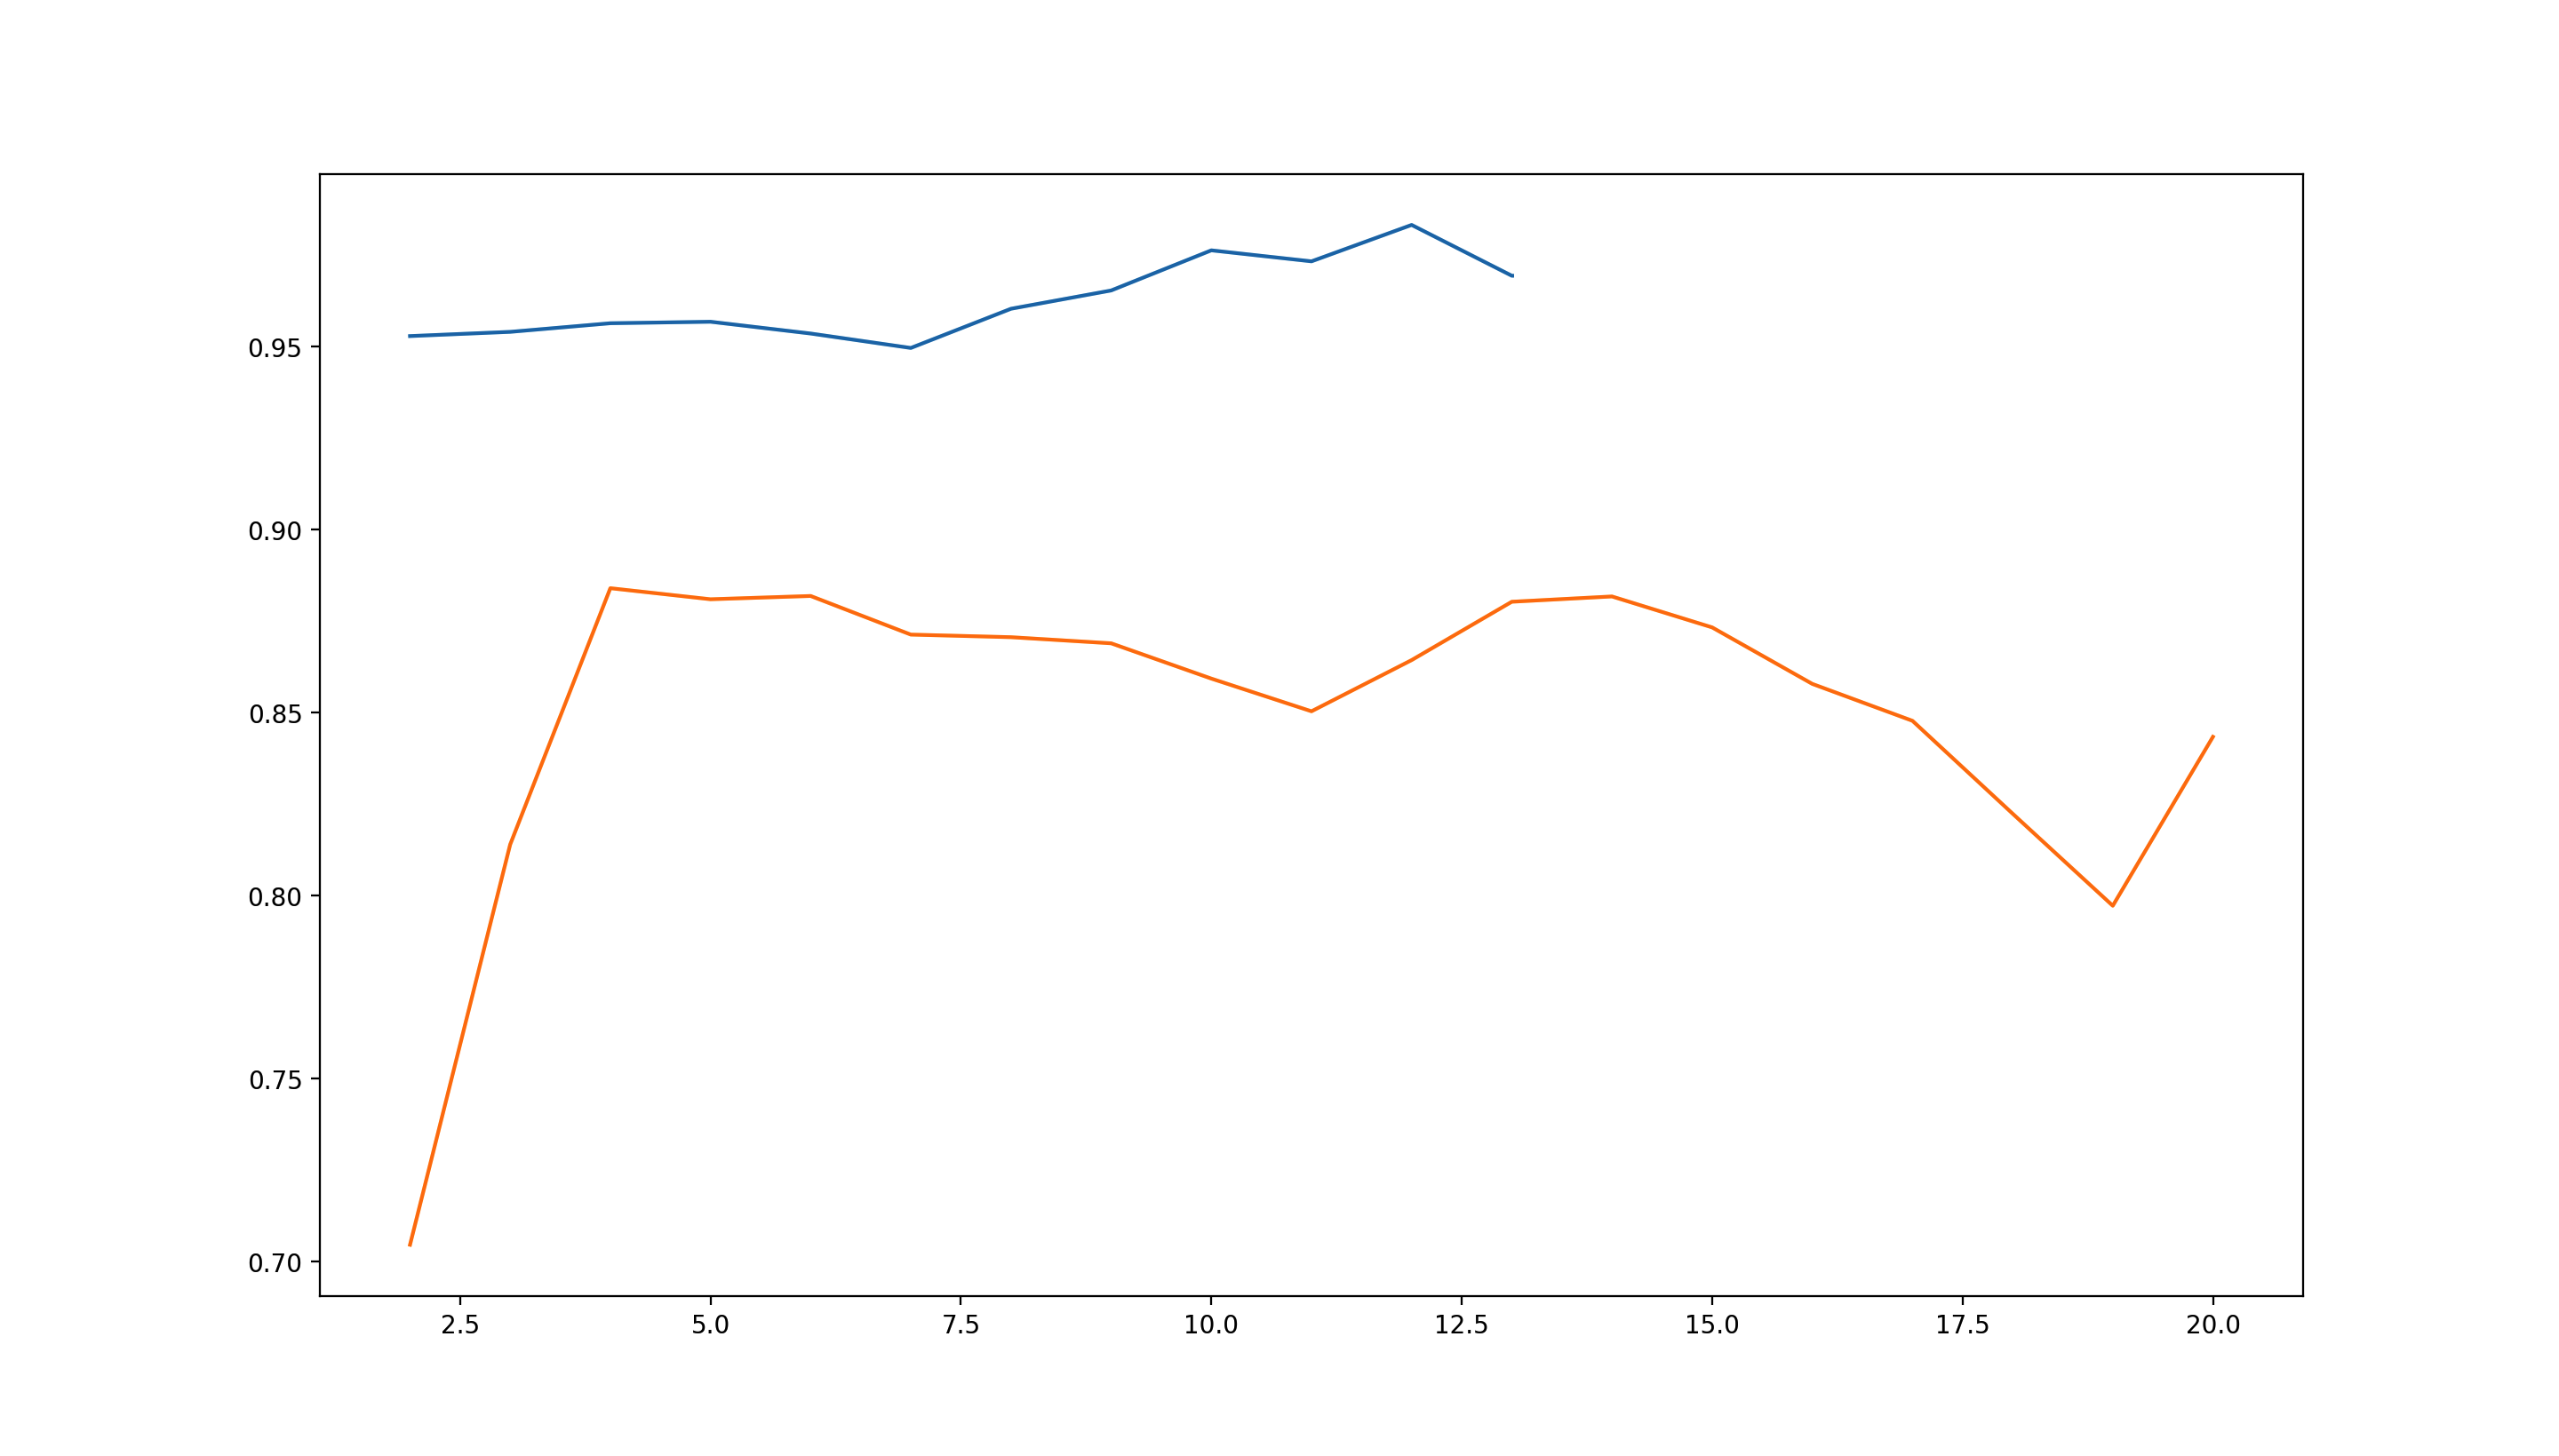
\includegraphics[width=\linewidth]{immagini/traintestrate.png}
	\caption{Accuracy in funzione del numero di giorni utilizzati come trainset. In blu è riportata l'accuracy del dataset A, in arancione quella del dataset B}
	\label{fig:traintestrate}
	\end{figure}

	\subsection{Analisi dei risultati}

	\subsubsection{Misure di qualità utilizzate}

	L'esecuzione dell'algoritmo di Viterbi su una sequenza di osservazioni, ha permesso di generare una sequenza di stati nascosti che, con una maggiore probabilità, ha portato alla realizzazione delle osservazioni date come input all'algoritmo.

	Una volta ottenuta la sequenza di stati frutto della previsione da parte dell'algoritmo di Viterbi, è stato possibile effettuare il confronto tra quest'ultima e la sequenza di stati reali, in modo da determinare la qualità dei risultati ottenuti.

	Per svolgere il controllo della qualità dei risultati sono stati testati i seguenti parametri:

	\begin{itemize}
		\item Accuracy
		\item Precision
		\item Recall
		\item F-Measure
	\end{itemize}

	Il test sulla Accuracy permette di trovare la percentuale di correttezza della sequenza di stati nascosti prevista. Di conseguenze, esprime, data una generica posizione i all'interno della sequenza di stati, se l'i-esimo stato nascosto previsto dall'algoritmo coincide con quello reale.

	Prima di descrivere le misure seguenti, è utile introdurre i termini vero positivo, vero negativo, falso positivo e falso negativo, i quali sono usati per confrontare la previsione dell'i-esimo stato nascosto rispetto il corretto stato alla posizione desiderata. Ad esempio:

	\begin{itemize}
		\item Vero positivo: l'i-esimo elemento corretto è sleeping e l'algoritmo ha predetto sleeping
		\item Vero negativo: l'i-esimo elemento corretto non è sleeping e l'algoritmo ha predetto non sleeping
		\item Falso positivo: l'i-esimo elemento corretto non è sleeping e l'algoritmo ha predetto sleeping
		\item Falso negativo: l'i-esimo elemento corretto è sleeping e l'algoritmo ha predetto non sleeping
	\end{itemize}

	A questo punto è possibile introdurre le ultime misure di test; Precision e Recall verranno quindi definiti come segue:

	\begin{center}
		$ Precision = \dfrac{Veropositivo}{VeroPositivo + Falsopositivo} $
	\end{center}

	\begin{center}
		$ Recall = \dfrac{Veropositivo}{VeroPositivo + Falsonegativo} $
	\end{center}

	Infine, il test F-Measure permette di misurare l'accuratezza di un test, attraverso l'uso di Precision e Recall, ed è descritto dalla formula:

		\begin{center}
		$ F-Measure = 2 * \dfrac{Precision * Recall}{Precision + Recall} $
	\end{center}



	\subsubsection{Capacità predittiva del modello}

	Per valutare la capacità predittiva del modello abbiamo svolto tre sperimentazioni diverse, tutte basandosi sul modello generato utilizzando come trainset i primi cinque giorni di osservazione di ognuno dei dataset (per i motivi citati precedentemente). Gli esperimenti svolti sono i seguenti:
	\begin{enumerate}
	    \item Predizione su un sottoinsieme del testset comprendente solo i primi tre giorni successivi ai giorni contenuti nel trainset.
	    \item Predizione sul testset nella sua interezza, ovvero dal giorno successivo al termine del trainset all'ultimo giorno di rilevazioni.
	    \item Predizione su un campione generato casualmente basandosi sulle distribuzioni di probabilità osservate nel dataset.
	\end{enumerate}

	\paragraph{Predizione a breve termine}

	Come anticipato in precedenza nella prima coppia di test effettuati sono stati utilizzati, per allenare il modello, i primi cinque giorni contenuti nel dataset, sia per il test su A, sia per il test su B; inoltre, il modello è stato testato in entrambi i casi attraverso la sequenza di osservazioni rilevate nei tre giorni seguenti, ovvero dal sesto all'ottavo giorno. Le matrici di confusione ottenute sono riportate in figura \ref{fig:a_3d} per il dataset A e in figura \ref{fig:b_3d} per il dataset b. Mentre in tabella \ref{tab:a_3d} e \ref{tab:b_3d} sono riportate le misure di Precision, Recall ed F-Measure rispettivamente per i dataset A e B.

    Per quanto riguarda il dataset A, la sequenza di stati predetta presenta un valore di \textbf{accuracy di 0,949}; ciò indica che la sequenza di stati che l'algoritmo ha predetto è molto simile a quella reale.

    Dalla tabella \ref{tab:a_3d} e dalla figura \ref{fig:a_3d}, si possono notare sia gli stati in cui l'algoritmo di Viterbi ha fornito una previsione migliore, sia quelli in cui l'algoritmo è stato meno preciso. Come si può dedurre, nella sequenza prevista dall'algoritmo, gli stati 2, 4, 5, 6 e 7 presentano un livello di predizione pressochè perfetto; mentre gli stati 0, 1, 3, 8 e 9 presentano una minore accuratezza; infatti nella sequenza prevista, questi vengono spesso scambiati, rispettivamente, con i valori 9, 8, 9, 9 e 7.

    Per quanto riguarda il dataset B, la sequenza di stati predetta presenta un valore di \textbf{accuracy di 0,927}; ciò indica che la sequenza di stati che l'algoritmo ha predetto è molto simile a quella reale, anche se ad un livello minore di A.

    Anche in questo caso, dalla tabella \ref{tab:b_3d} e dalla figura \ref{fig:b_3d}, si possono notare sia gli stati in cui l'algoritmo di Viterbi ha fornito una previsione migliore, sia quelli in cui l'algoritmo è stato meno preciso.

    In questo dataset, a differenza del caso precedente, la maggior parte degli stati viene prevista con un buon livello di accuratezza, infatti la maggior parte di essi viene predetto correttamente con una probabilità maggiore o uguale di 0,8. Ciò non vale per gli stati 0, che viene spesso scambiato con lo stato 10, e soprattutto con lo stato 7, il quale non viene mai previsto correttamente.

    Da questo esperimento è possibile affermare che il modello creato è in grado di effettuare una previsione dettagliata di una sequenza di stati nascosti, utilizzando una sequenza di osservazioni. Ciò è presumibilmente dovuto al fatto che la combinazione di osservazioni, rappresentate dai bit di sensori attivi in una timeslice, è in grado di identificare in modo preciso una determinata attività, rendendone possibile la previsione.

	\begin{figure}[!htbp]
	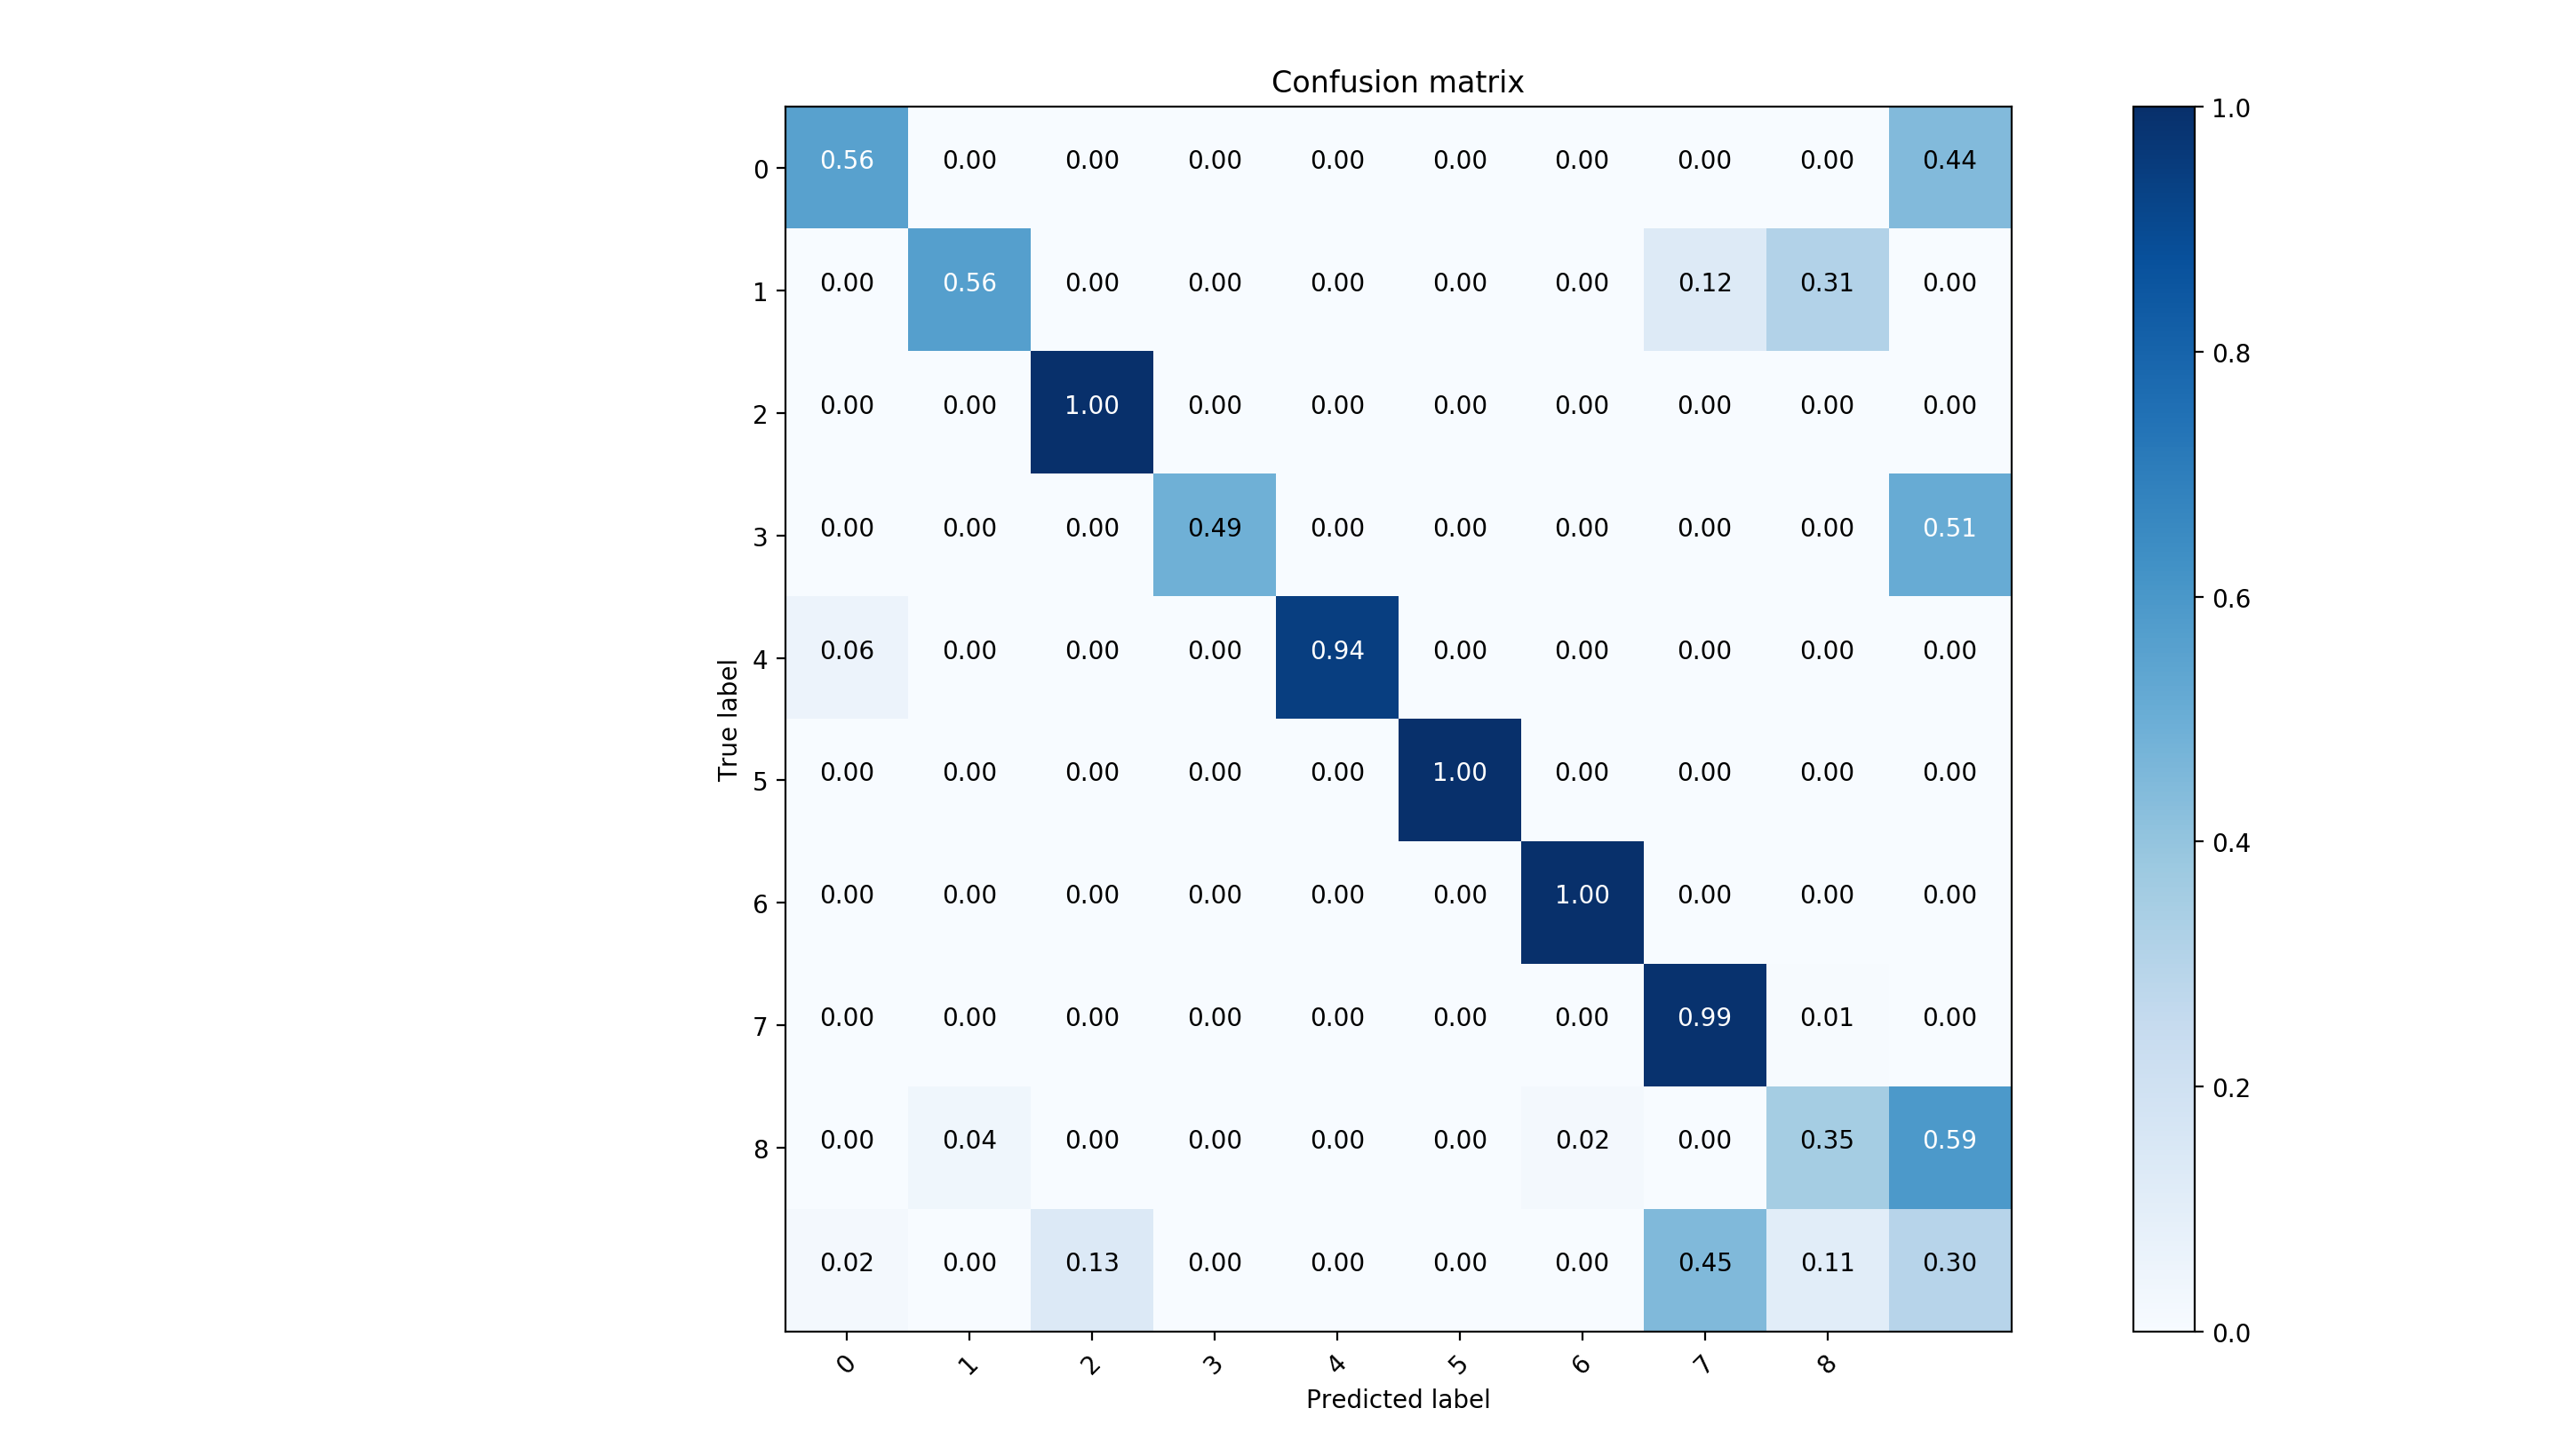
\includegraphics[width=\linewidth]{immagini/confusion_matrix/a_3d.png}
	\caption{Matrice di confusione per il dataset A, testset di 3 giorni}
	\label{fig:a_3d}
	\end{figure}

	\begin{figure}[!htbp]
	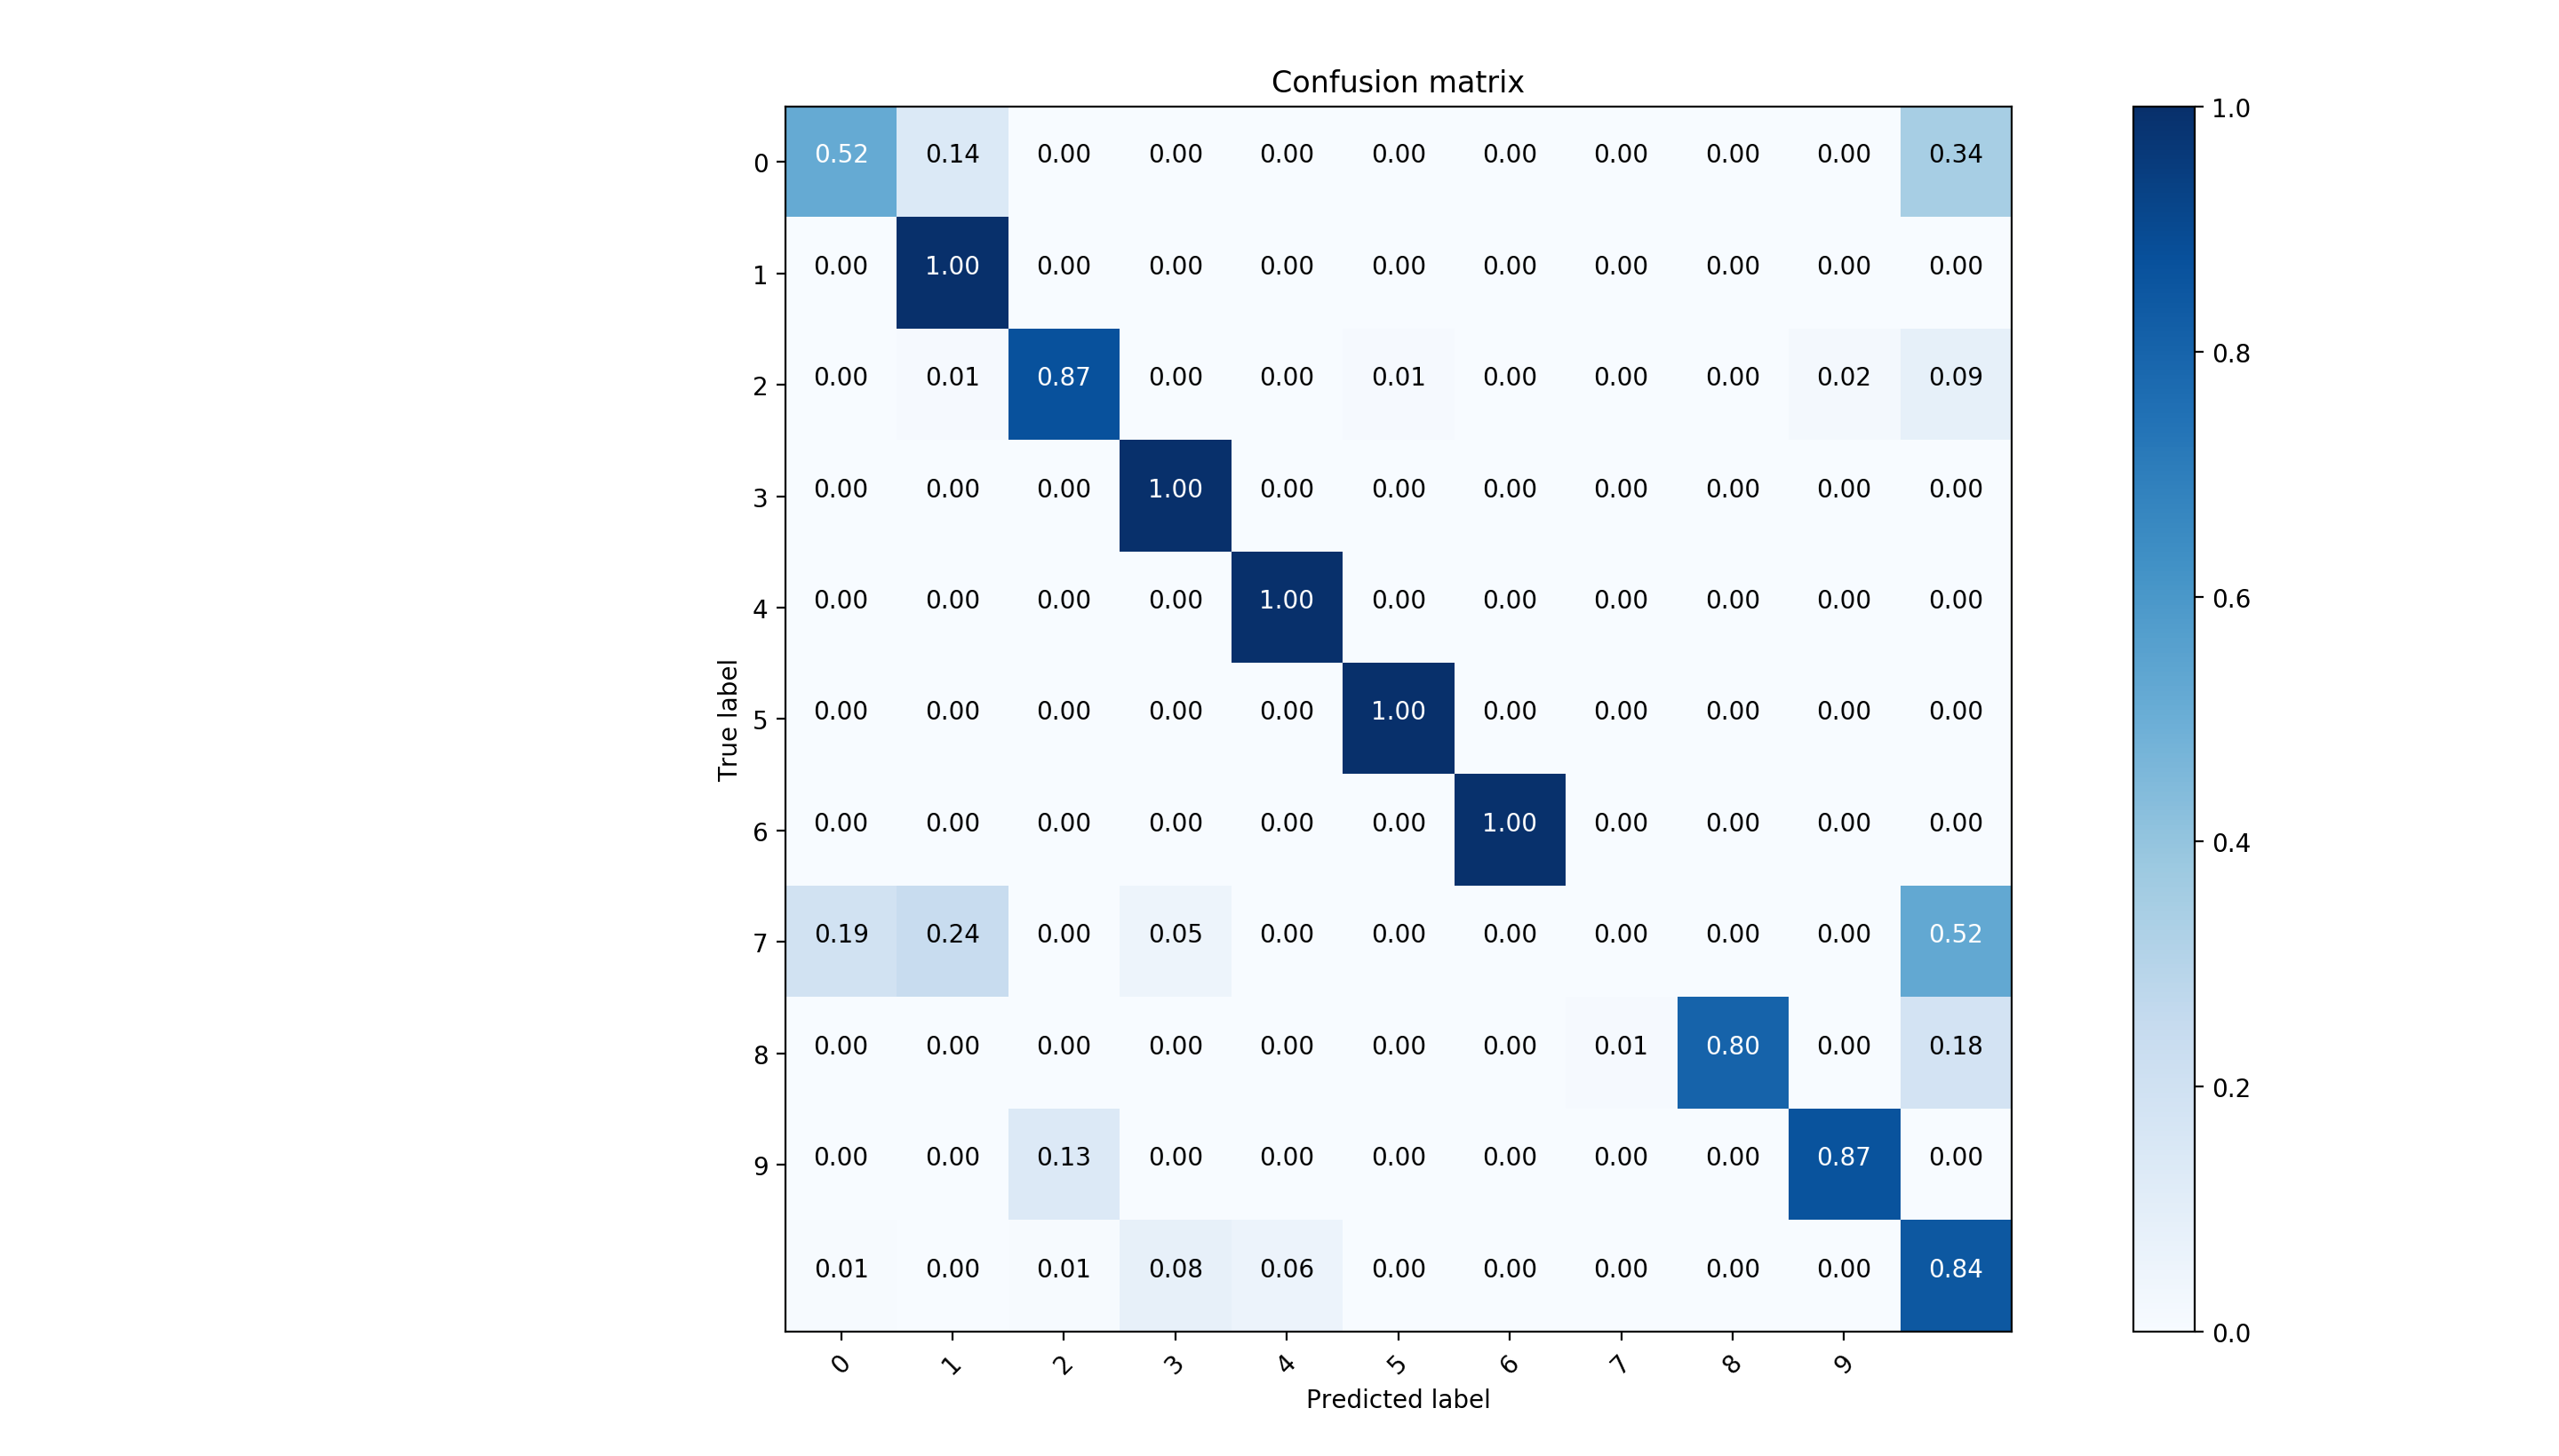
\includegraphics[width=\linewidth]{immagini/confusion_matrix/b_3d.png}
	\caption{Matrice di confusione per il dataset B, testset di 3 giorni}
	\label{fig:b_3d}
	\end{figure}


	\begin{table}[!htbp]
    \scriptsize
    \centering
    	\begin{tabularx}{0.56\textwidth}{l | llll}
    		{} & {precision} & {recall} & {f1-score} & {support} \\
    		\midrule
            {0} & {0.79} & {0.56} & {0.65} & {27} \\
            {1} & {0.75} & {0.56} & {0.64} & {16} \\
            {2} & {0.95} & {1.00} & {0.98} & {471} \\
            {3} & {1.00} & {0.49} & {0.66} & {45} \\
            {4} & {1.00} & {0.94} & {0.97} & {18} \\
            {5} & {1.00} & {1.00} & {1.00} & {1783} \\
            {6} & {0.25} & {1.00} & {0.40} & {1} \\
            {7} & {0.95} & {0.99} & {0.97} & {1726} \\
            {8} & {0.34} & {0.35} & {0.35} & {54} \\
            {9} & {0.44} & {0.30} & {0.35} & {179} \\
            {avg/total} & {0.94} & {0.95} & {0.94} & {4320} \\
    	\end{tabularx}
    	\captionof{table} {Misure di Precision, Recall ed F-Measure per il dataset A, trainset di 3 giorni}
    	\label{tab:a_3d}
    \end{table}

	\begin{table}[!htbp]
    \scriptsize
    \centering
    	\begin{tabularx}{0.56\textwidth}{l | llll}
    		{} & {precision} & {recall} & {f1-score} & {support} \\
    		\midrule
            {0} & {0.68} & {0.52} & {0.59} & {29} \\
            {1} & {0.18} & {1.00} & {0.30} & {3} \\
            {2} & {0.89} & {0.87} & {0.88} & {94} \\
            {3} & {0.97} & {1.00} & {0.98} & {1219} \\
            {4} & {0.60} & {1.00} & {0.75} & {45} \\
            {5} & {0.94} & {1.00} & {0.97} & {15} \\
            {6} & {1.00} & {1.00} & {1.00} & {1452} \\
            {7} & {0.00} & {0.00} & {0.00} & {21} \\
            {8} & {1.00} & {0.80} & {0.89} & {899} \\
            {9} & {0.81} & {0.87} & {0.84} & {15} \\
            {10} & {0.69} & {0.84} & {0.76} & {528} \\
            {avg/total} & {0.94} & {0.93} & {0.93} & {4320} \\
    	\end{tabularx}
    	\captionof{table} {Misure di Precision, Recall ed F-Measure per il dataset B, trainset di 3 giorni}
    	\label{tab:b_3d}
    \end{table}



	\paragraph{Predizione a lungo termine}

	Nella seconda coppia di test effettuati sono stati utilizzati, per allenare il modello, i primi cinque giorni contenuti nel dataset, sia per il test su A, sia per il test su B; inoltre, il modello è stato testato in entrambi i casi attraverso la sequenza di osservazioni rilevate seguenti, ovvero dal sesto al quattordicesimo giorno nel caso di A, e dal sesto al ventunesimo giorno nel caso di B. Le matrici di confusione ottenute sono riportate in figura \ref{fig:a_9d} per il dataset A e in figura \ref{fig:b_16d} per il dataset b. Mentre in tabella \ref{tab:a_9d} e \ref{tab:b_16d} sono riportate le misure di Precision, Recall ed F-Measure rispettivamente per i dataset A e B.

	Per quanto riguarda il dataset A, la sequenza di stati predetta presenta un valore di \textbf{accuracy di 0,957}; ciò indica che la sequenza di stati che l'algoritmo ha predetto è più simile a quella reale rispetto a quella del test precedente.

	Dalla tabella \ref{tab:a_9d} e dalla figura \ref{fig:a_9d}, si possono notare sia gli stati in cui l'algoritmo di Viterbi ha fornito una previsione migliore, sia quelli in cui l'algoritmo è stato meno preciso. In questo test, cinque stati sono stati previsti correttamente con un livello di accuratezza pari o superiore a 0,8. Bisogna sottolineare come, tra gli stati che hanno ottenuto un punteggio minore, non vi è più lo stato 1; tuttavia a questo gruppo si è aggiunto lo stato 6, che presenta una precisione di previsione molto più bassa rispetto al precedente test.

    Per quanto riguarda il dataset B, la sequenza di stati predetta presenta un valore di \textbf{accuracy di 0,891}; ciò indica che la sequenza di stati che l'algoritmo ha predetto è molto simile a quella reale, tuttavia in minore quantità rispetto a quella ottenuta nel test precedente .

    Anche in questo caso, dalla tabella \ref{tab:b_16d} e dalla figura \ref{fig:b_16d}, si possono notare sia gli stati in cui l'algoritmo di Viterbi ha fornito una previsione migliore, sia quelli in cui l'algoritmo è stato meno preciso.

    In questo dataset, a differenza del caso di A, tutti gli stati vengono previsti con un livello di accuratezza simile a quello ottenuto nel primo esperimento; tuttavia è presente una generale diminuzione della precisione con la quale è avvenuta la previsione, che permette di spiegare il minor valore di accuracy ottenuto in questo caso.

    Da questo esperimento è possibile dedurre che il modello è in grado di effettuare la previsione di una sequenza di stati, data una sequenza di osservazioni. Più precisamente, è stato ottenuto un risultato migliore sul dataset riguardante l'abitazione A, mentre il dataset dell'abitazione B ha portato a risultati leggermente peggiori.



	\begin{figure}[!htbp]
	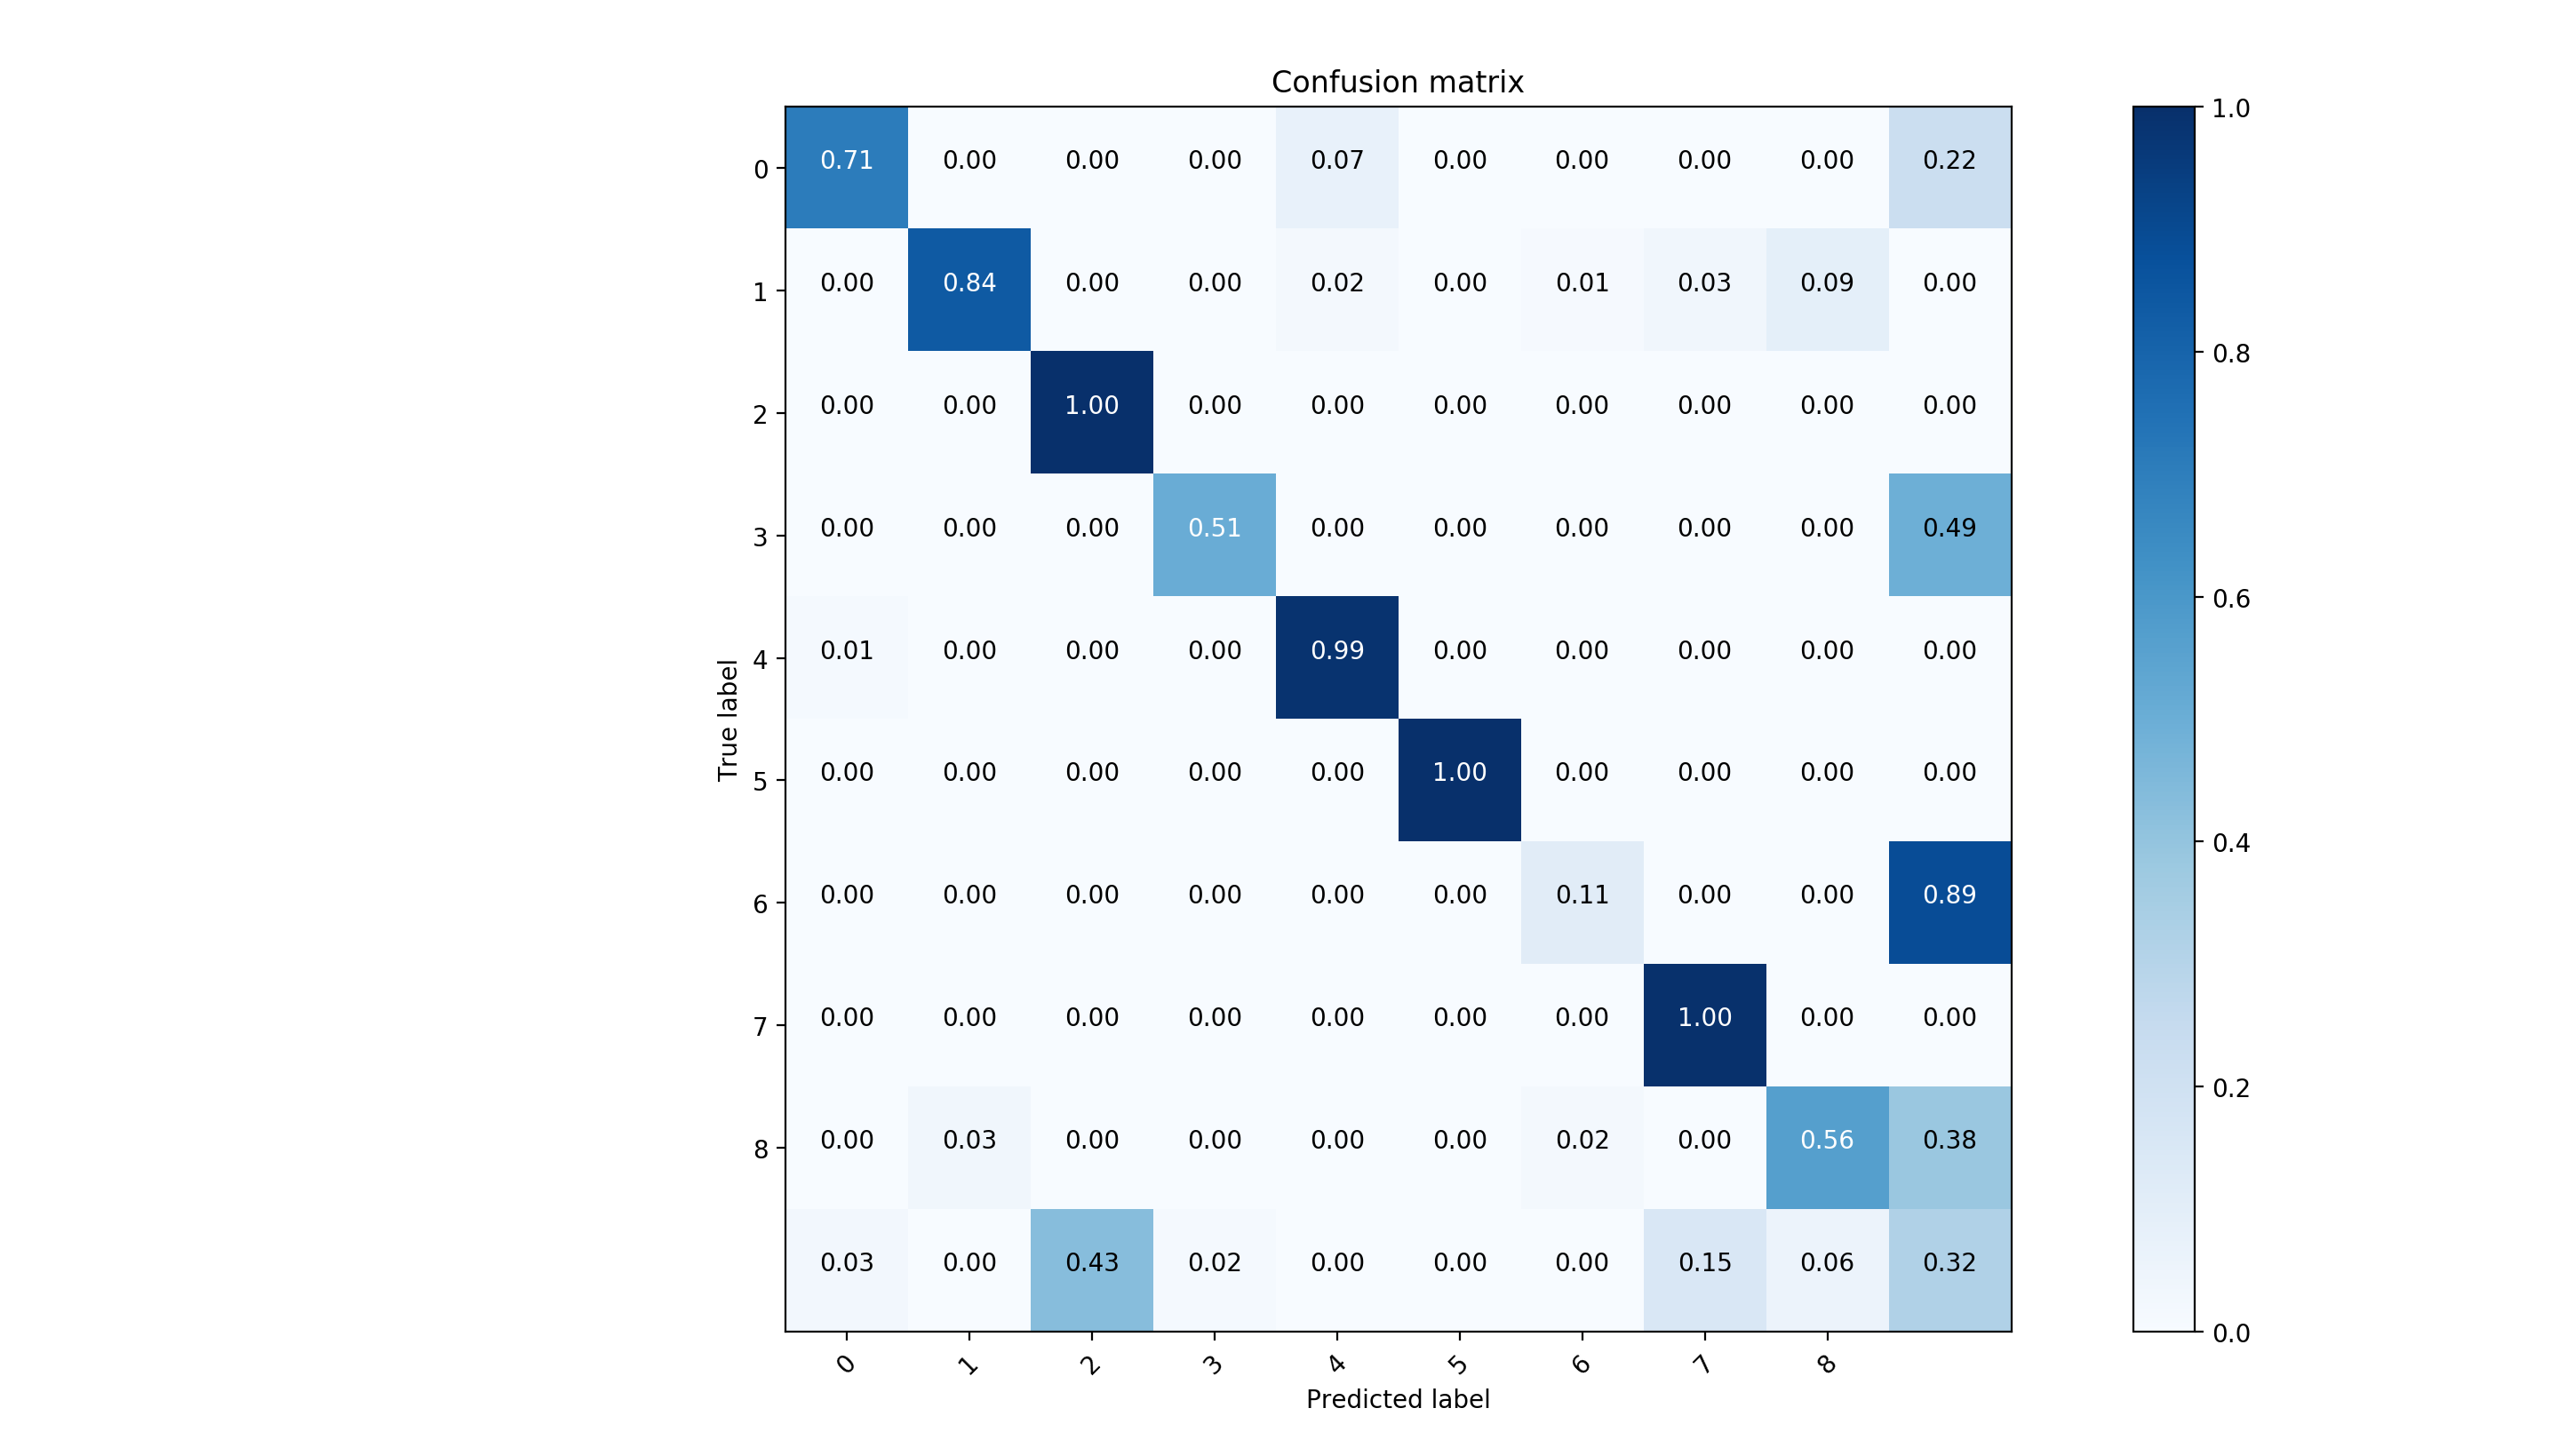
\includegraphics[width=\linewidth]{immagini/confusion_matrix/a_10d.png}
	\caption{Matrice di confusione per il dataset A, testset di 9 giorni}
	\label{fig:a_9d}
	\end{figure}

	\begin{figure}[!htbp]
	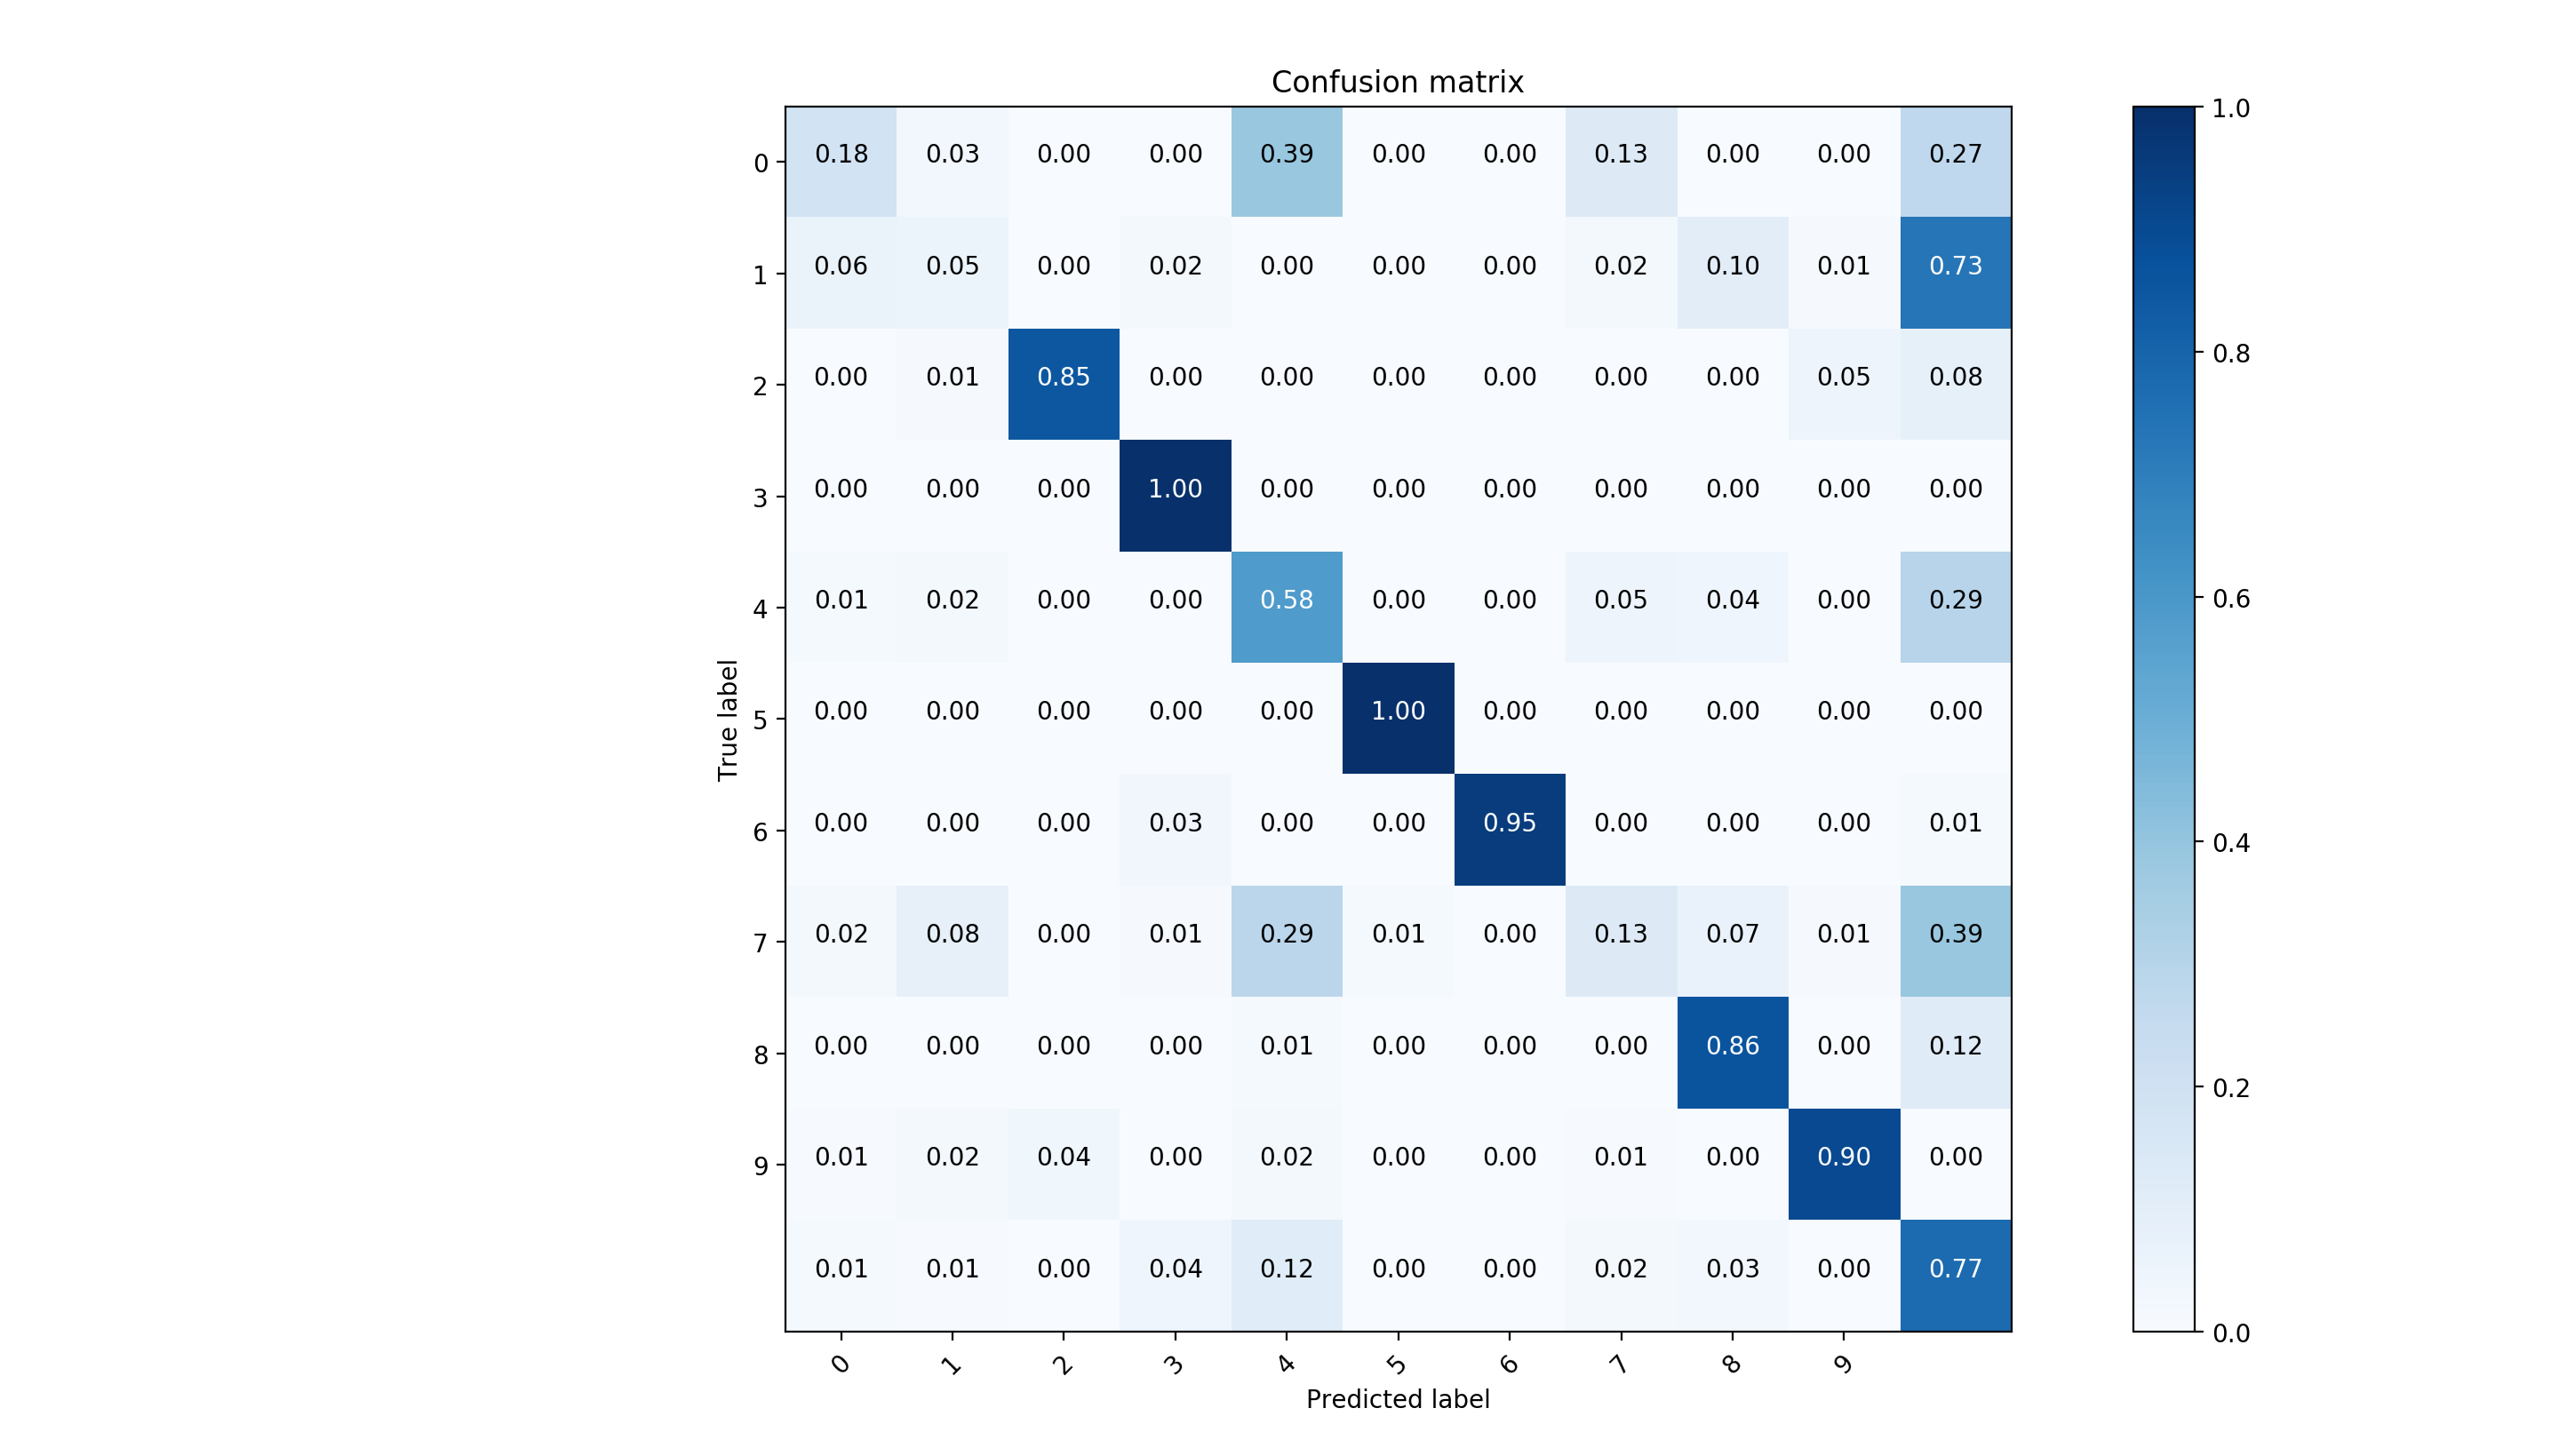
\includegraphics[width=\linewidth]{immagini/confusion_matrix/b_16d.png}
	\caption{Matrice di confusione per il dataset B, testset di 16 giorni}
	\label{fig:b_16d}
	\end{figure}


	\begin{table}[!htbp]
    \scriptsize
    \centering
    	\begin{tabularx}{0.56\textwidth}{l | llll}
    		{} & {precision} & {recall} & {f1-score} & {support} \\
    		\midrule
            {0} & {0.80} & {0.71} & {0.75} & {85} \\
            {1} & {0.94} & {0.84} & {0.88} & {87} \\
            {2} & {0.87} & {1.00} & {0.93} & {1474} \\
            {3} & {0.92} & {0.51} & {0.65} & {174} \\
            {4} & {0.90} & {0.99} & {0.94} & {72} \\
            {5} & {1.00} & {1.00} & {1.00} & {5170} \\
            {6} & {0.14} & {0.11} & {0.12} & {9} \\
            {7} & {0.98} & {1.00} & {0.99} & {5263} \\
            {8} & {0.50} & {0.56} & {0.53} & {94} \\
            {9} & {0.53} & {0.32} & {0.40} & {532} \\
            {avg/total} & {0.95} & {0.96} & {0.95} & {12960} \\
    	\end{tabularx}
    	\captionof{table} {Misure di Precision, Recall ed F-Measure per il dataset A, trainset di 9 giorni}
    	\label{tab:a_9d}
    \end{table}

	\begin{table}[!htbp]
    \scriptsize
    \centering
    	\begin{tabularx}{0.56\textwidth}{l | llll}
    		{} & {precision} & {recall} & {f1-score} & {support} \\
    		\midrule
            {0} & {0.48} & {0.18} & {0.27} & {234} \\
            {1} & {0.07} & {0.05} & {0.06} & {96} \\
            {2} & {0.93} & {0.85} & {0.89} & {320} \\
            {3} & {0.92} & {1.00} & {0.96} & {4417} \\
            {4} & {0.19} & {0.58} & {0.28} & {211} \\
            {5} & {0.93} & {1.00} & {0.96} & {63} \\
            {6} & {1.00} & {0.95} & {0.97} & {8353} \\
            {7} & {0.18} & {0.13} & {0.15} & {214} \\
            {8} & {0.98} & {0.86} & {0.92} & {6514} \\
            {9} & {0.77} & {0.90} & {0.83} & {129} \\
            {10} & {0.61} & {0.77} & {0.68} & {2489} \\
            {avg/total} & {0.91} & {0.89} & {0.90} & {23040} \\
    	\end{tabularx}
    	\captionof{table} {Misure di Precision, Recall ed F-Measure per il dataset B, trainset di 16 giorni}
    	\label{tab:b_16d}
    \end{table}

	\paragraph{Predizione con campione casuale}

	Nell'ultima coppia di test effettuati sono stati utilizzati, per allenare il modello, i primi cinque giorni contenuti nel dataset, sia per il test su A, sia per il test su B; inoltre, il modello è stato testato in entrambi i casi attraverso la sequenza di osservazioni generate a caso, contenenti 3000 minuti. Le matrici di confusione ottenute sono riportate in figura \ref{fig:a_3ks} per il dataset A e in figura \ref{fig:b_3ks} per il dataset b. Mentre in tabella \ref{tab:a_3ks} e \ref{tab:b_3ks} sono riportate le misure di Precision, Recall ed F-Measure rispettivamente per i dataset A e B.

	In quest'ultimo esperimento sono stati ottenuti i migliori valori di accuracy, ovvero \textbf{accuracy di 0,968} per il dataset A e \textbf{accuracy di 0.914} per il dataset B.

	Dalle tabelle \ref{tab:a_3ks} e \ref{tab:b_3ks} e dalle figure \ref{fig:a_3ks} e \ref{fig:b_3ks}, si possono notare gli stati che sono stati predetti con una maggiore accuratezza.

	I valori migliori di accuratezza ottenuti in questo esperimento erano prevedibili, in quanto il campione generato si basa sulle matrici ricavate dal trainset utilizzato per allenare il modello, di conseguenza vengono emesse, anche se in modo randomico, delle sequenze facilmente prevedibili dal modello.




	\begin{figure}[!htbp]
	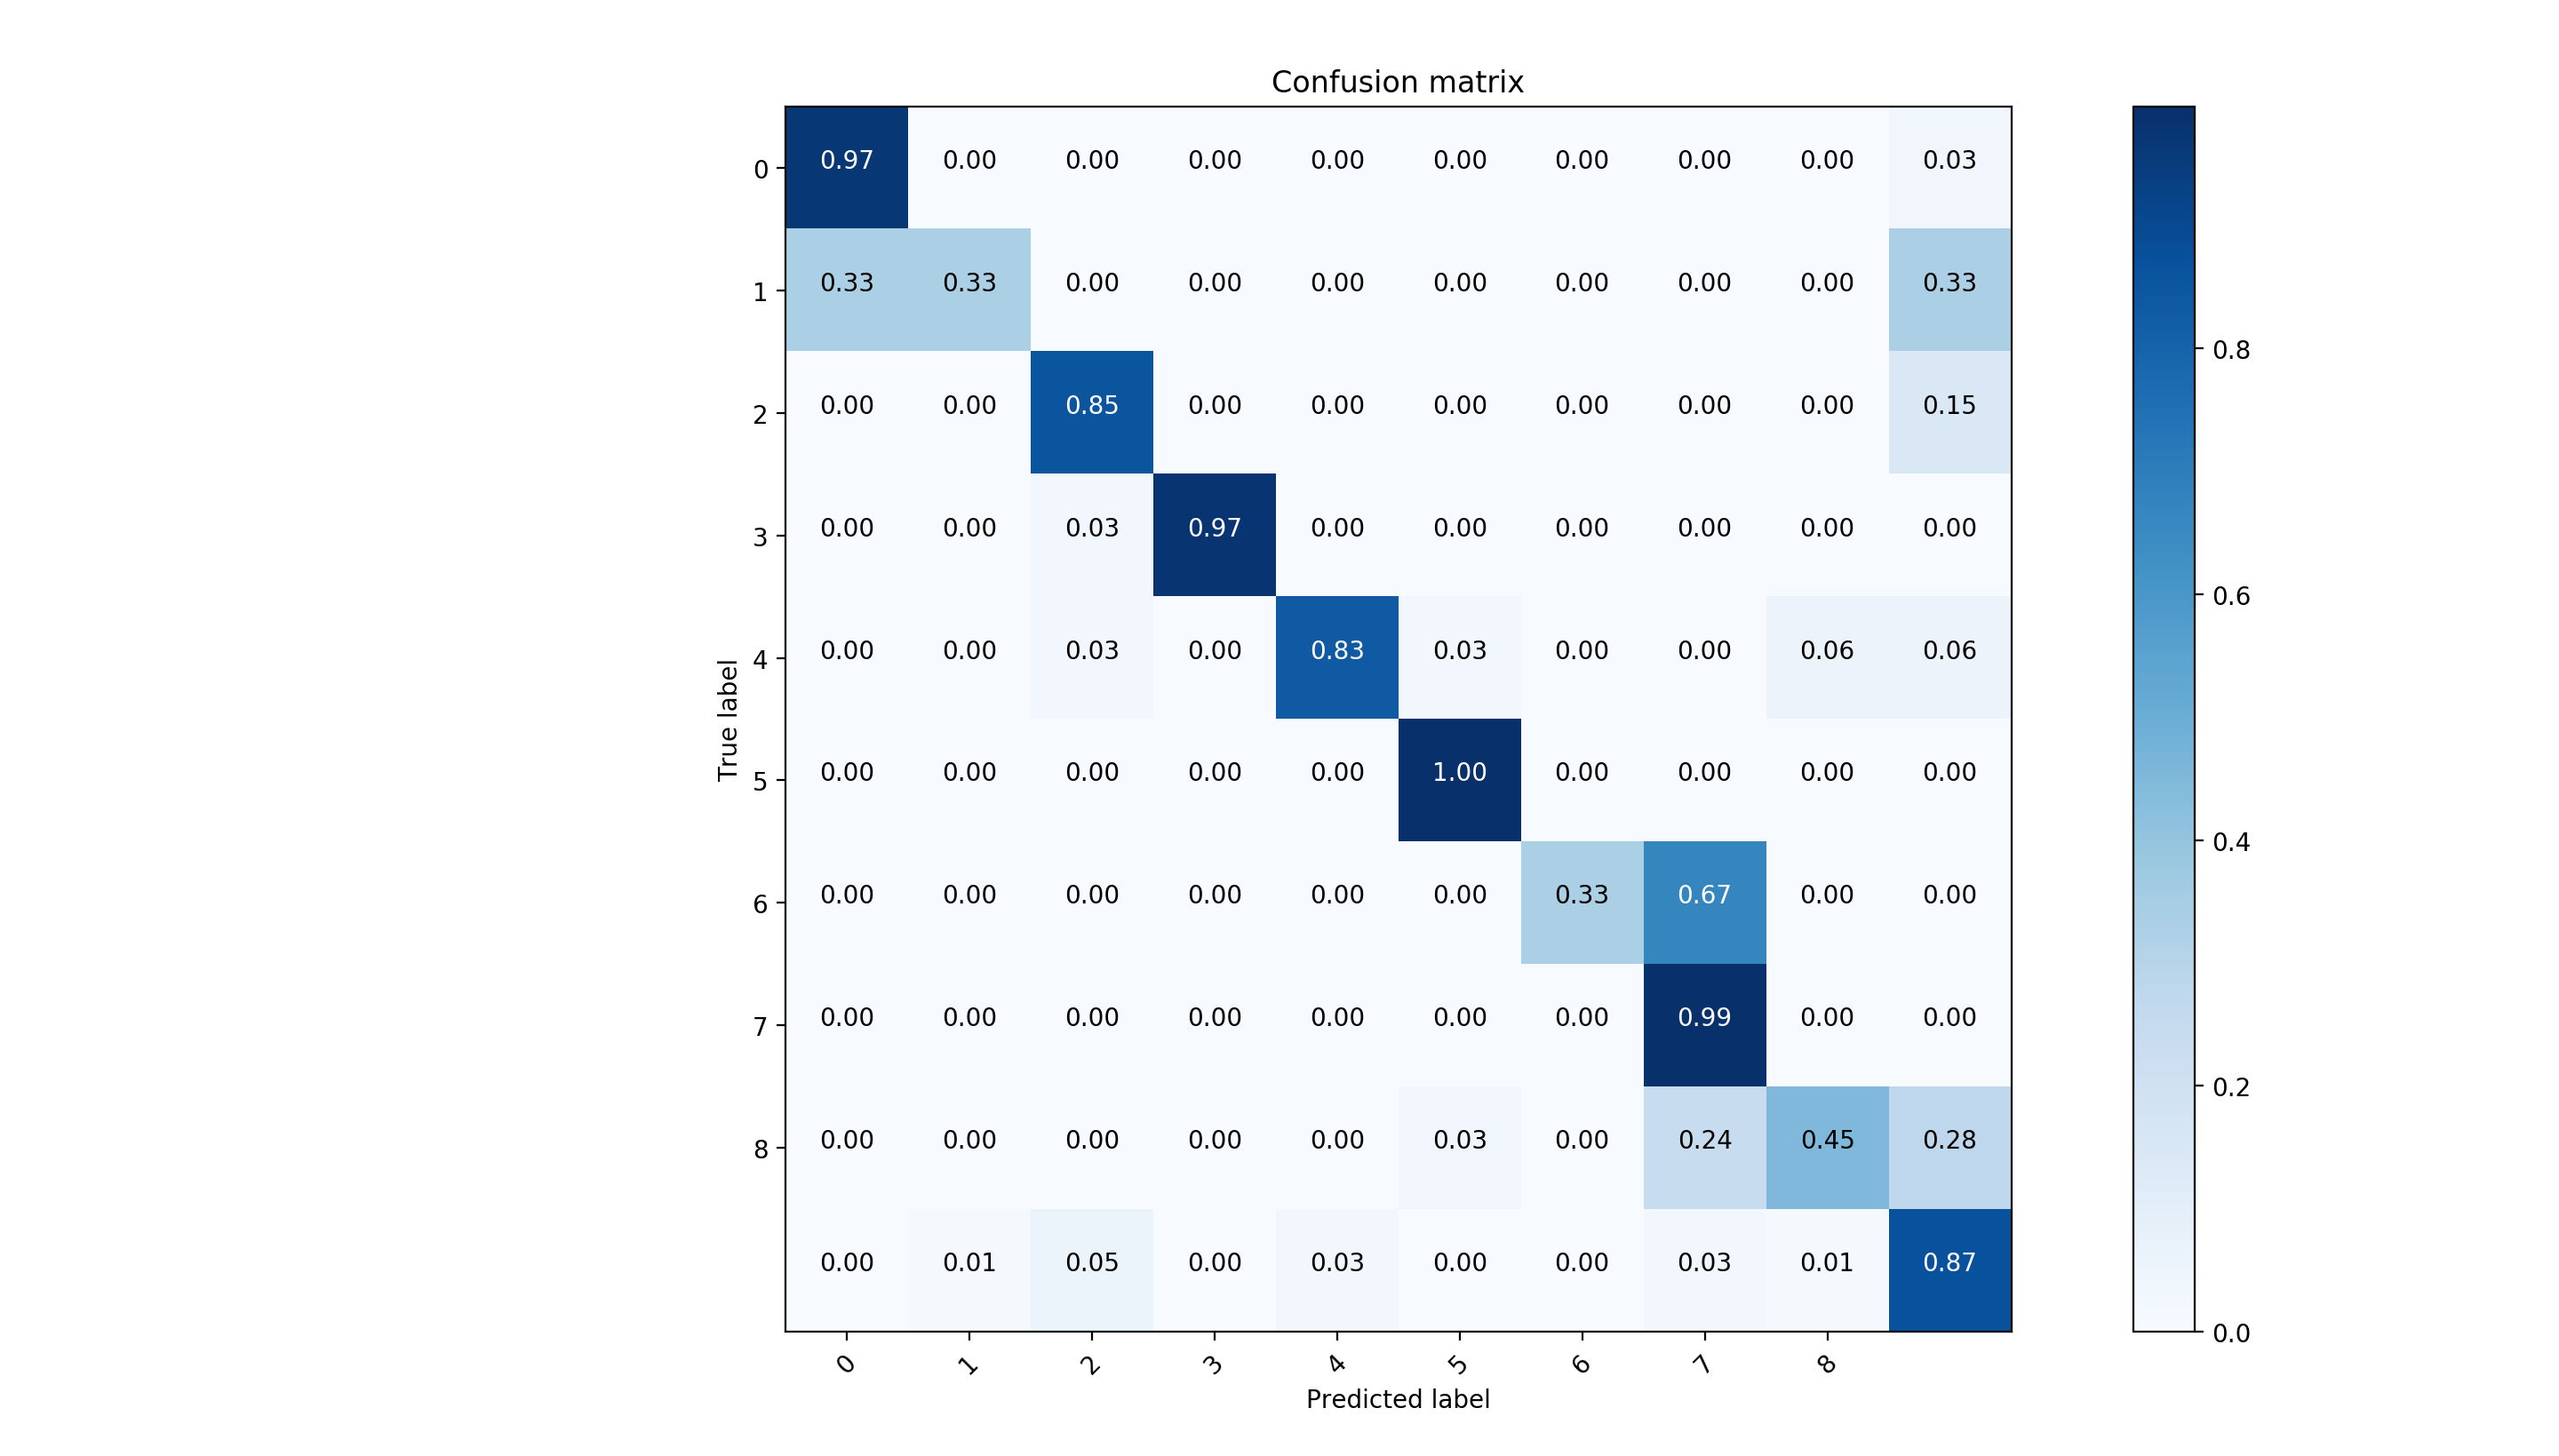
\includegraphics[width=\linewidth]{immagini/confusion_matrix/a_3ks.png}
	\caption{Matrice di confusione per il dataset A, testset casuale di 3000 campioni}
	\label{fig:a_3ks}
	\end{figure}

	\begin{figure}[!htbp]
	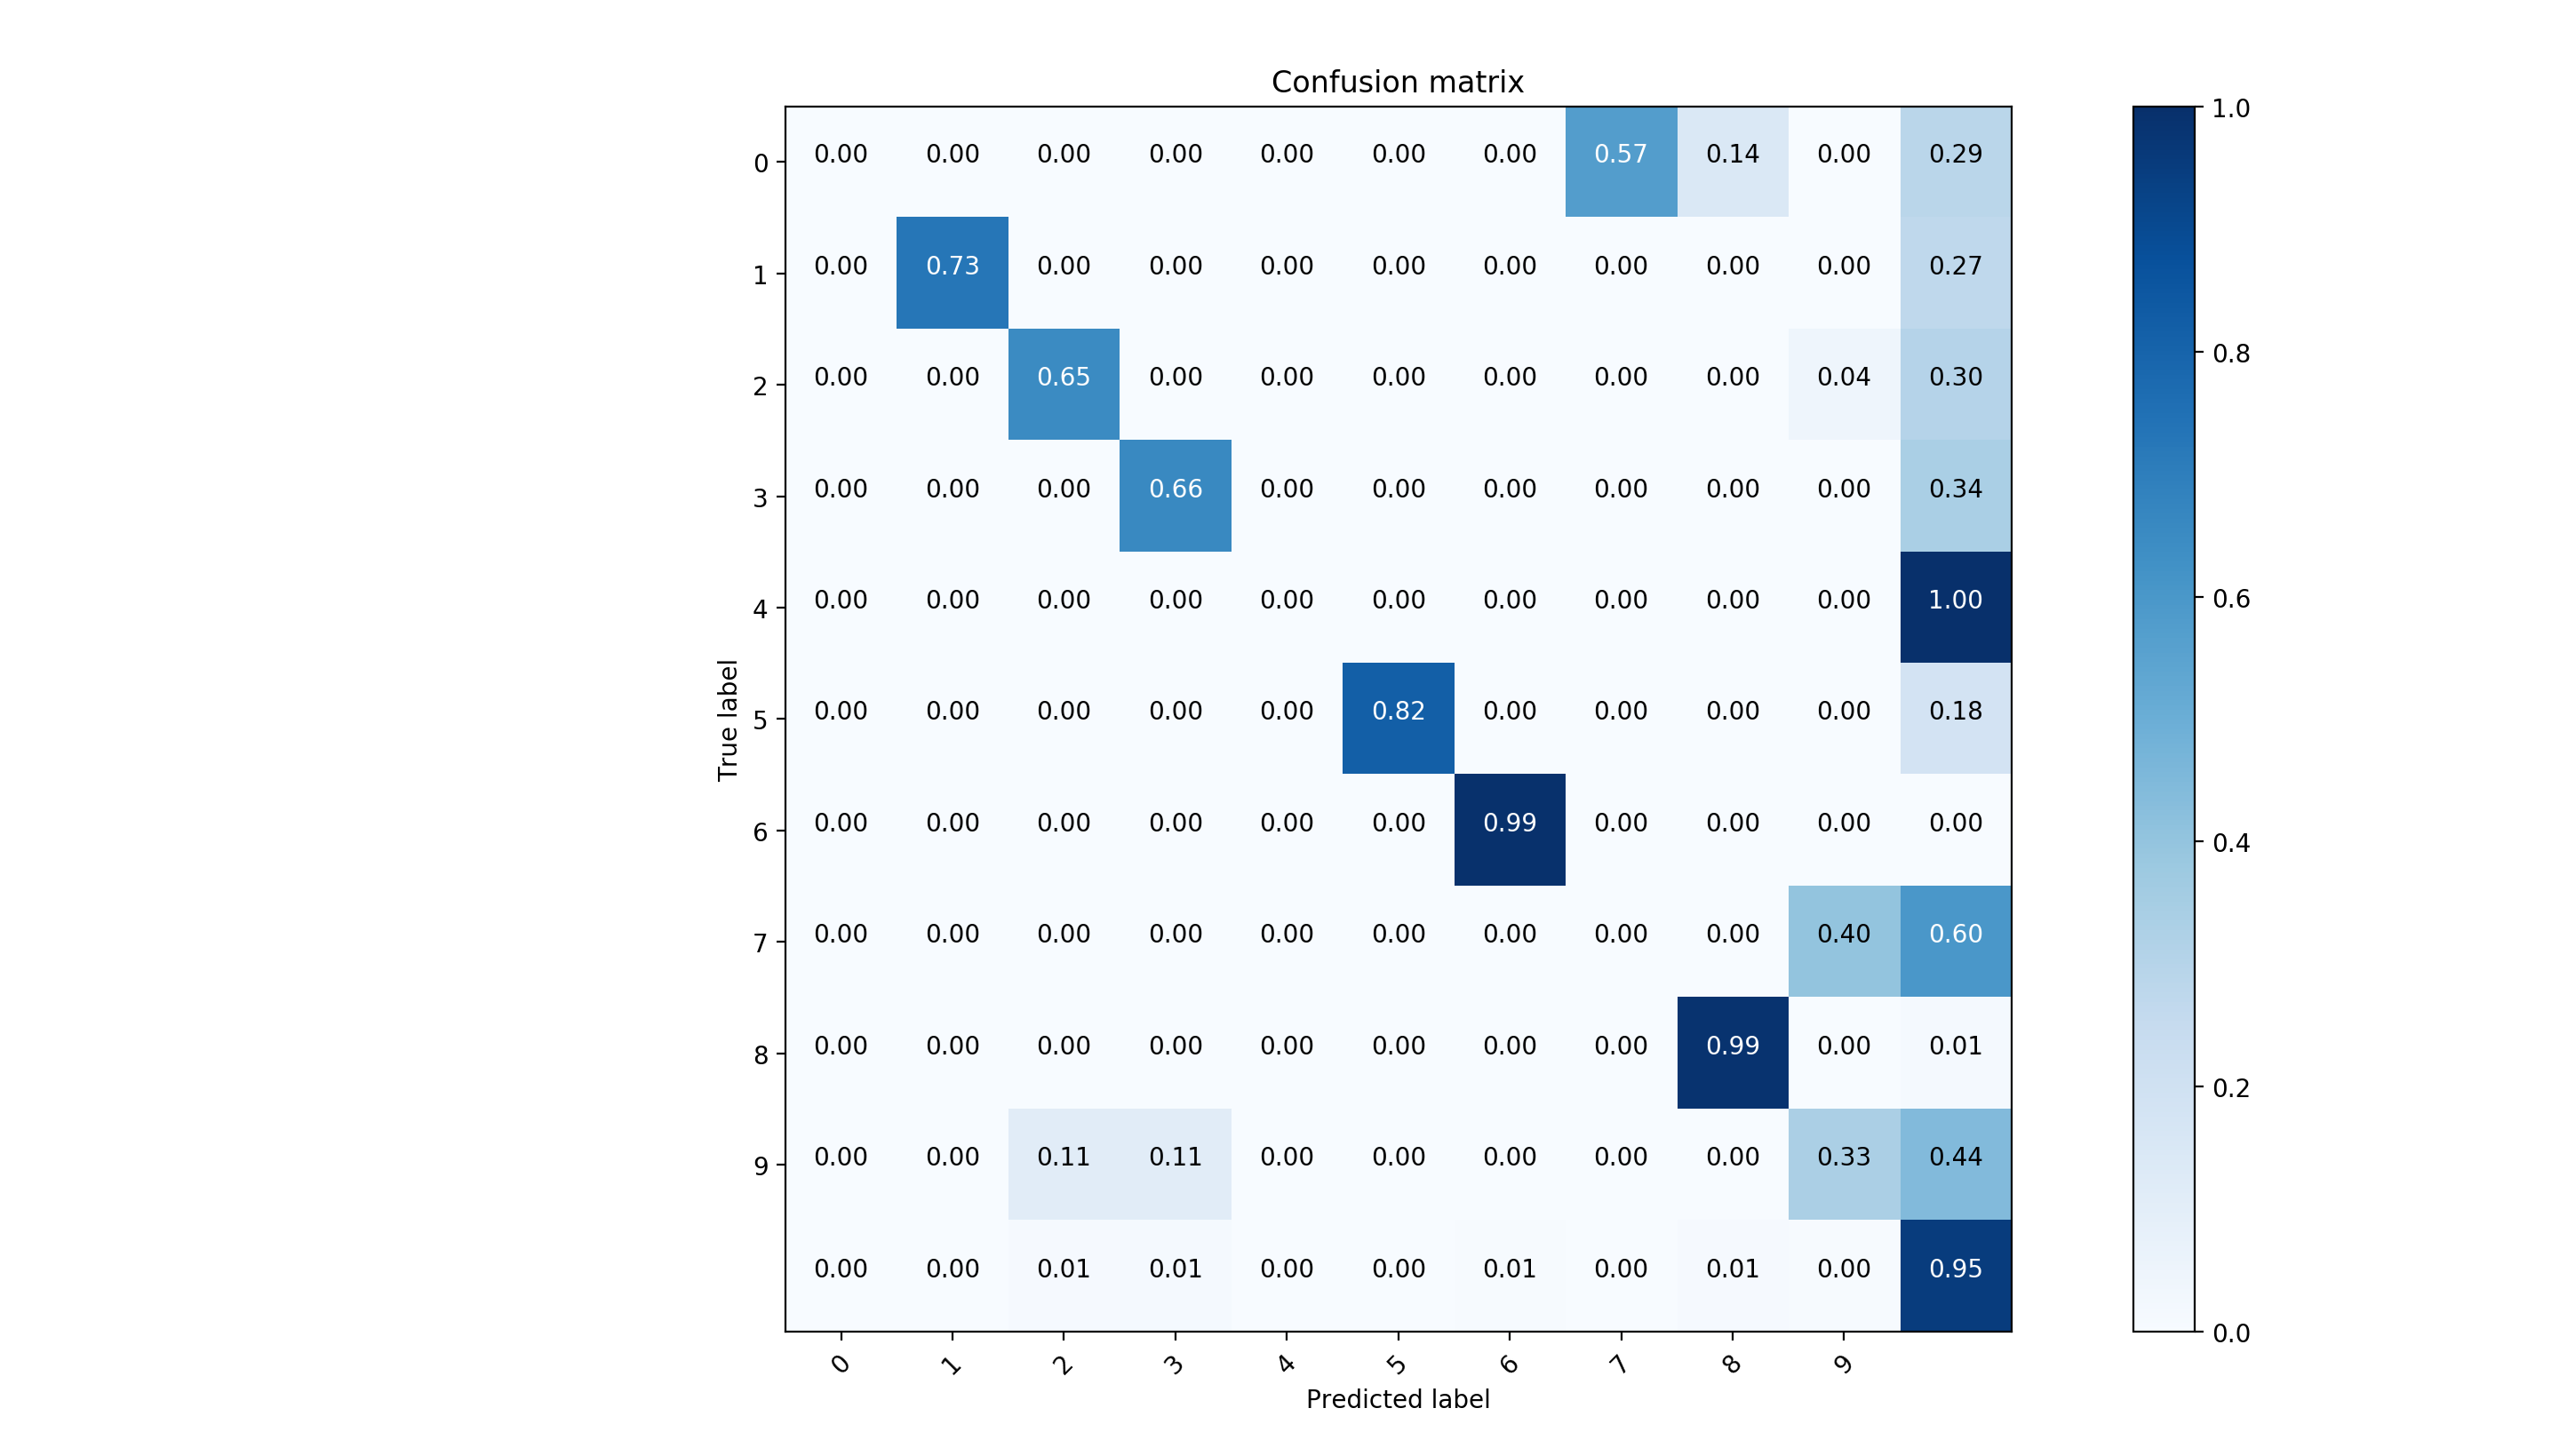
\includegraphics[width=\linewidth]{immagini/confusion_matrix/b_3ks.png}
	\caption{Matrice di confusione per il dataset B, testset di 3000 campioni}
	\label{fig:b_3ks}
	\end{figure}


	\begin{table}[!htbp]
    \scriptsize
    \centering
    	\begin{tabularx}{0.56\textwidth}{l | llll}
    		{} & {precision} & {recall} & {f1-score} & {support} \\
    		\midrule
            {0} & {0.97} & {0.97} & {0.97} & {30} \\
            {1} & {0.20} & {0.33} & {0.25} & {3} \\
            {2} & {0.89} & {0.85} & {0.87} & {137} \\
            {3} & {0.97} & {0.97} & {0.97} & {116} \\
            {4} & {0.83} & {0.83} & {0.83} & {36} \\
            {5} & {1.00} & {1.00} & {1.00} & {640} \\
            {6} & {0.33} & {0.33} & {0.33} & {3} \\
            {7} & {0.99} & {0.99} & {0.99} & {1790} \\
            {8} & {0.62} & {0.45} & {0.52} & {29} \\
            {9} & {0.83} & {0.87} & {0.85} & {216} \\
            {avg/total} & {0.97} & {0.97} & {0.97} & {3000} \\
    	\end{tabularx}
    	\captionof{table} {Misure di Precision, Recall ed F-Measure per il dataset A, testset casuale di 3000 campioni}
    	\label{tab:a_3ks}
    \end{table}

	\begin{table}[!htbp]
    \scriptsize
    \centering
    	\begin{tabularx}{0.56\textwidth}{l | llll}
    		{} & {precision} & {recall} & {f1-score} & {support} \\
    		\midrule
{ 0} & {1.00} & {0.87} & {0.93} & {  52} \\
{ 1} & {0.80} & {0.80} & {0.80} & {   5} \\
{ 2} & {0.76} & {0.81} & {0.79} & {  48} \\
{ 3} & {0.82} & {0.73} & {0.77} & { 393} \\
{ 6} & {1.00} & {1.00} & {1.00} & {1055} \\
{ 7} & {1.00} & {0.67} & {0.80} & {  48} \\
{ 8} & {0.98} & {0.98} & {0.98} & { 765} \\
{ 9} & {0.15} & {0.15} & {0.15} & {  13} \\
{10} & {0.78} & {0.86} & {0.82} & { 621} \\
{avg/total} & {0.92} & {0.91} & {0.91} & {3000} \\
    	\end{tabularx}
    	\captionof{table} {Misure di Precision, Recall ed F-Measure per il dataset B, testset casuale di 3000 campioni}
    	\label{tab:b_3ks}
    \end{table}


	\section{GUI}

	\begin{figure}[!htbp]
	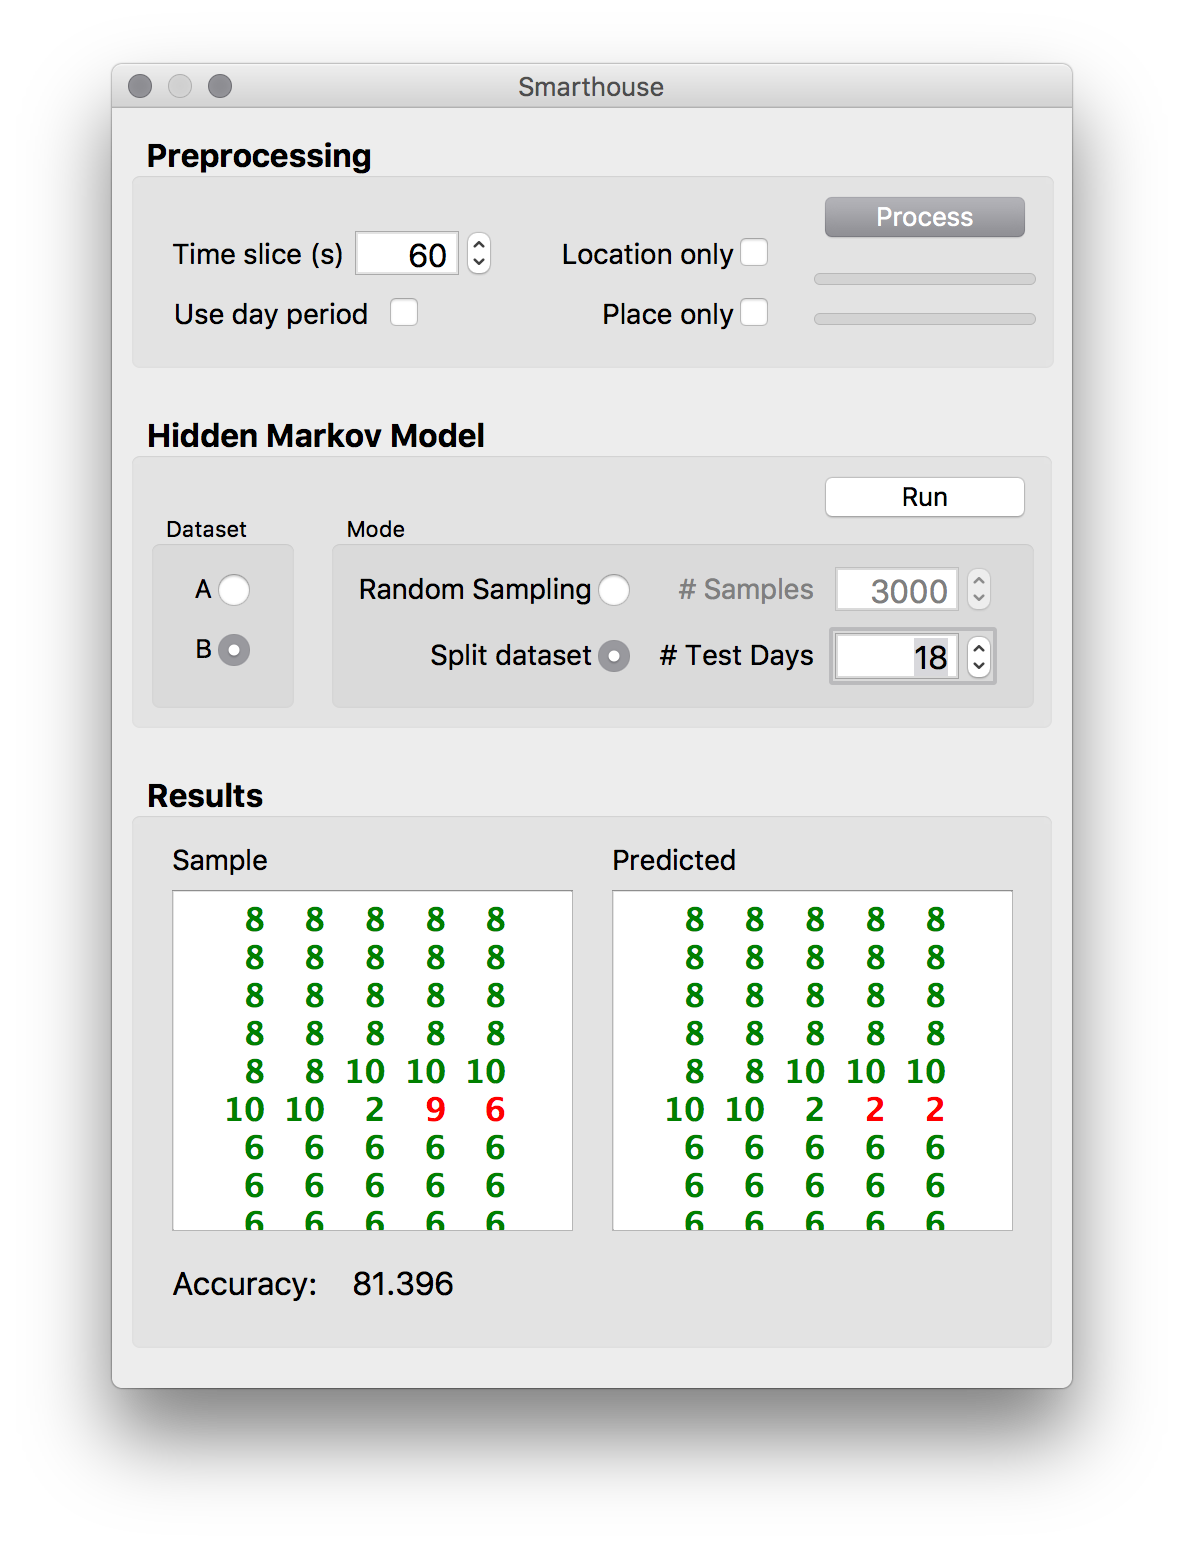
\includegraphics[width=\linewidth]{immagini/gui.png}
	\caption{Interfaccia grafica}
	\label{fig:b_3ks}
	\end{figure}
	\begin{itemize}
	    \item Punto A: sezione per precisare l'ampiezza del timeslice. In questa sezione possono essere settati dei parametri riguardanti il preprocessing dei dati, dedicati alla scelta delle colonne del dataset da utilizzare per identificare ogni istanza
	    \item Punto B: sezione dedicata alla scelta del dataset da utilizzare
	    \item Punto C: sezione dedicata alle modalità con cui eseguire il test; è possibile scegliere se testare il modello sulla divisione in testset e trainser oppure se utilizzare una sequenza generata randomicamente. Inoltre è possibile settare anche la lunghezza, in giorni, del testset o il numero delle istanze da generare randomicamente.
	    \item Punto D: sezione in cui vengono presentati i risultati, nel riquadro a sinistra è presente la sequenza di stati corretta, mentre sulla destra quella predetta. Ogni stato è colorato di verde, nel caso sia stato predetto correttamente, rosso se viceversa. In basso viene presentato il valore di accuracy riscontrato.
	\end{itemize}


	\clearpage
	\section{Conclusioni}

	In questa relazione è stato creato e discusso un modello HMM collocato nell'ambito del servizio sanitario; questo modello, infatti, è stato creato attraverso dei dati ottenuti grazie alle rilevazioni di attività e di sensori all'interno di alcune abitazioni di anziani. Quest'ambito di ricerca è molto importante, in quanto un netto miglioramento delle tecnologie in ambito medico ha portato ad un conseguente innalzamento dell'età media di un individuo. La presenza di tecnologie in grado di rilevare le attività all'interno di un'abitazione quindi, permette la sicurezza degli individui più anziani, promuovendone l'autonomia.

	Nella relazione svolta, è stata prima svolta la presentazione del dataset utilizzato per la creazione dell'Hidden Markov Model, a cui è seguita la creazione di quest'ultimo.
	Nell'ultima parte, è stata invece descritta la sperimentazione eseguita, della quale ne sono stati discussi i risultati.

	Il modello risulta essere eccessivamente accurato anche con solo pochi giorni di training, e sembra mostrare dell'overfitting sui dati . Questo ipotizziamo sia dovuto al fatto che la routine della giornata è poco variabile e quindi sono sufficienti pochi giorni di osservazione per avere buone previsioni. Inoltre il modello non prevedere gli stati con la stessa precisione, infatti le attività che mediamente durano di più vengono previste con estrema facilità, mentre quelle più brevi hanno precisioni molto inferiori. Infine abbiamo notato un forte bias nel predirre lo stato relativo a "Nessuna attività".
\end{document}
